\documentclass[
  utf8,%     More capable input encoding than latin-1.
  % parskip,%  For vertical whitespace between paragraphs.  This comes down to more than just using parskip.sty, so it's better to use this class option.
  % S5MP % If you intend to really use margin paragraphs (not recommended!).
%  crop,%     Produce output with crop marks and paper size A4.  Liu-Tryck should like this.  Automatically adds information, including the physical page number, at the top of each page.
       %     Add option 'noInfo' to suppress the info at the top of each page when using option 'crop'.
  % Font options: 'kp' (default), 'times', 'lm'.  The KpFonts (loaded using 'kp'), is the most complete font among the provided options.  Among other, it supports slanted small caps.  See rtthesis.cls for more details regarding the font options.
  largesmallcaps,intlimits,widermath,% Good options to KpFonts.
  sharecounter,nobreak,definition=marks,%  See comments in the results chapter of this document for more information on these options!
  numbers, % If you want to cite references by numbers, use this option.
  noparts% Use option 'noparts' if you do not make use of part divisions.
]{rtthesis}

\usepackage{mythesis}

\documentclass{article}

\usepackage[style=ieee,backend=biber]{biblatex}
\addbibresource{./bibtex/bib/cite.bib}


\usepackage[margin=3cm]{geometry}
\usepackage[utf8]{inputenc}
\usepackage{color}
\usepackage[]{todonotes}
\usepackage{amsmath}
\usepackage{float}
\usepackage{graphicx} % Allow graphics.
\usepackage{csquotes}
\usepackage{tikz} 
\usepackage{nonfloat}
\usepackage[ampersand]{easylist}
\usepackage{pdfpages}
\usepackage{subcaption}
\usepackage{caption}
%\usepackage{subfig}
\usepackage{mathrsfs,amsmath}
\usepackage{fancyhdr}
\usepackage{listings}
\usepackage{placeins}   

\usepackage{amsfonts}
% or
%\usepackage{amssymb}

\usepackage{listings}
\usepackage{color}

\usepackage{amsthm}
 
\theoremstyle{definition}
\newtheorem{definition}{Definition}[]
 
\theoremstyle{remark}
\newtheorem*{remark}{Remark}
 
\definecolor{codegreen}{rgb}{0,0.6,0}
\definecolor{codegray}{rgb}{0.5,0.5,0.5}
\definecolor{codepurple}{rgb}{0.58,0,0.82}
\definecolor{backcolour}{rgb}{0.95,0.95,0.92}
 
\lstdefinestyle{mystyle}{
    backgroundcolor=\color{backcolour},   
    commentstyle=\color{codegreen},
    keywordstyle=\color{magenta},
    numberstyle=\tiny\color{codegray},
    stringstyle=\color{codepurple},
    basicstyle=\footnotesize,
    breakatwhitespace=false,         
    breaklines=true,                 
    captionpos=b,                    
    keepspaces=true,                 
    numbers=left,                    
    numbersep=5pt,                  
    showspaces=false,                
    showstringspaces=false,
    showtabs=false,                  
    tabsize=2
}
 
\lstset{style=mystyle}
 
 
%%
\usepackage{nomencl}
\makenomenclature

%% This removes the main title:
\renewcommand{\nomname}{}
%% this modifies item separation:
\setlength{\nomitemsep}{8pt}
%% this part defines the groups:
%----------------------------------------------
\usepackage{etoolbox}
\renewcommand\nomgroup[1]{%
  \item[\Large\bfseries
  \ifstrequal{#1}{N}{Nomenclature}{%
  \ifstrequal{#1}{A}{List of Abbreviations}{}}%
]\vspace{10pt}} % this is to add vertical space between the groups.
%----------------------------------------------

\usepackage{subcaption}
\begin{document}
\selectlanguage{english}

\frontmatter
\maketitle

\begin{abstract}[swedish]
  Foton tagna i det korta infraröda spektrumet är intressanta i militära sammanhang på grund av att de är mindre beroende av vilken tid på dygnet de är tagna för att solen, månen, stjärnor och nattsken (night glow) lyser upp jorden med kortvågiga infraröd strålning dynget runt. Ett stort problem med dagens kortvågig infraröda kameror är att de är väldigt dyra att producera och därav inte tillgängliga till en bred skara, varken militärt eller civilt. Med hjälp av en relativt ny teknik kallad \textit{compressive sensing} (CS) möjligörs en ny typ av kamera med endast en pixel i sensorn. Denna nya typ av kamera behöver bara en bråkdel mätningar relativt antal pixlar som ska återskapas och reducerar kostnaden på en kortvågig infraröd kamera med en faktor 20. Kameran använder en mikrospegelmatris som används för att välja vilka speglar (pixlar) som ska mätas i scenen och på så sätt skapa ett underbestämt ekvationssystem som kan lösas med teknikerna beskrivna i CS för att återskapa bilden. Givet den nya tekniken är det i Totalförsvarets forskningsinstituts (FOI) intresse att utvärdera potentialen hos en enpixel-kamera. Med en enpixel-kameraarkitektur utvecklad av FOI var målet med detta examensarbete att ta fram metoder för att sampla, återskapa bilder och utvärdera deras kvalitet. Detta examensarbete visar att användning av strukturella slumpade matriser och snabba transformer öppnar upp för högupplösta bilder och snabbar upp processen att rekonstruera bilder avsevärt. Utvärderingen av bilderna kunde göras med vanliga mått associerade med kamerautvärdering och visade att kameran kan återskapa högupplösta bilder med relativt hög bildkvalitet i dagsljus. \citep{article:FOI_pres_sens}
\end{abstract}

\begin{abstract}[english]
  

Photos captured in the shortwave infrared (SWIR) spectrum are interesting in military applications because they are independent of what time of day the picture is captured because the sun, moon, stars and night glow illuminate the earth with short-wave infrared radiation constantly. A major problem with today's SWIR cameras is that they are very expensive to produce and hence not broadly available either within the military or to civilians. Using a relatively new technology called compressive sensing (CS), enables a new type of camera with only a single pixel sensor in the sensor (a SPC). This new type of camera only needs a fraction of measurements relative to the number of pixels to be reconstructed and reduces the cost of a short-wave infrared camera with a factor of 20. The camera uses a micromirror array (DMD) to select which mirrors (pixels) to be measured in the scene, thus creating an underdetermined linear equation system that can be solved using the techniques described in CS to reconstruct the image. Given the new technology, it is in the Swedish Defence Research Agency (FOI) interest to evaluate the potential of a single pixel camera. With a SPC architecture developed by FOI, the goal of this thesis was to develop methods for sampling, reconstructing images and evaluating their quality. This thesis shows that structured random matrices and fast transforms have to be used to enable high resolution images and speed up the process of reconstructing images significantly. The evaluation of the images could be done with standard measurements associated with camera evaluation and showed that the camera can reproduce high resolution images with relative high image quality in daylight.

\end{abstract}

\begin{acknowledgments}
 HELLO

  \addvspace{1em}
  \begin{flushright}
    \textit{%
      Link\"{o}ping, Januari 2018\\
      Andreas Brorsson%
    }
  \end{flushright}
\end{acknowledgments}


\tableofcontents
\begin{notation}% Passing the option "old" to the notation environment will redefine the notationtabular environment so that it produces an old style LaTeX tabular instead of a booktabs.sty style tabular.
  \centering

  \begin{notationtabular}{Nomenclature}{Notation}{Meaning}
    $\mathbf{y}$ & Measured signal \\
    $\mathbf{\Phi}$ & Measurement matrix  \\
    $\mathbf{x}$ & The spatial scene \\
    $\mathbf{\Psi}$ & Basis matrix \\
    $\mathbf{\theta}$ & Coefficients in basis $\Psi$ \\
    $\mathbf{A}$ & Sensing matrix in new basis \\
    $N$ & Number of reconstructed pixels \\
    $M$ & Number of single pixel measurements \\
    $\epsilon$ & Noise from measurements \\
  \end{notationtabular}

  \begin{notationtabular}{Abbreviations}{Abbreviations}{Meaning}
  	\abbrBRISQUE\index{BRISQUE@\abbrBRISQUE!abbreviation} & Blind/referenceless image spatial quality evaluator\\
    \abbrCS\index{CS@\abbrCS!abbreviation} & Compressive sensing \\
    \abbrCI\index{CS@\abbrCI!abbreviation} & Compressive imaging \\
    \abbrDLP\index{DLP@\abbrDLP!abbreviation} & Digital light processor\\
    \abbrDMD\index{DMD@\abbrDMD!abbreviation} & Digital micromirror device\\
    \abbrIID\index{IID@\abbrIID!abbreviation} & Independent and identically distributed \\
    \abbrFOI\index{FOI@\abbrFOI!abbreviation} & Swedish Defence Research Agency \\
    FWHT & Fast Walsh-Hadamard transform \\
    
    PSNR & Peak signal-to-noise ratio \\
    
    	\abbrRIP\index{RIP@\abbrRIP!abbreviation} & Restricted isometry
property\\
	\abbrSLM\index{SLM@\abbrSLM!abbreviation} &  Spatial Light Modulator\\
    \abbrSPC\index{SPC@\abbrSPC!abbreviation} & Single pixel camera\\

    \abbrSRM\index{SRM@\abbrSRM!abbreviation} & Structurally random
matrix\\

	SSIM & Structural similarity\\
	
	\abbrSWIR\index{SWIR@\abbrSWIR!abbreviation} & Short-wavelength infrared\\
	
	\abbrTV\index{TV@\abbrTV!abbreviation} & Total variation\\
	
  \end{notationtabular}
\end{notation}


\mainmatter
\section{Introduction}
The development and research of compressed sensing applied to a single pixel camera (SPC) is a relative new area in signal processing with the first functioning camera architecture in 2006. Since then numerous improvements and methods have been proposed how to capture images. In this section a introduction to the SPC architecture and a brief introduction of compressed imaging is presented followed by the aim, research questions and thesis outline. 

\subsection{Compressive sensing \& imaging}
Compressive sensing is a new sampling strategy which reconstructs a compressible or sparse signal by finding solution to undetermined linear system where the number of measurements $M$ is less then the number of data points $N$ in signal. Two constraints need to be fulfilled to apply compressed sensing sampling: the sampled signal needs to be spares in some basis e.g. Fourier or gradient, the second condition is that the measurement matrix must be incoherent with the sparse transform. The characteristic  undetermined linear system in CS is defined as $ \mathbf{y} = \mathbf{\Phi}\mathbf{x}$ where $\mathbf{y}$ contains the measurements from the measurement matrix $\mathbf{\Phi}$ sensing the signal $\mathbf{x}$. In figure~\ref{fig:CS_eq_sys} such linear equation system is shown.

\begin{figure}[H]
	\includegraphics[scale=0.5]{gfx/CS_eq.eps}
	\caption{CS undetermined linear system}
	\label{fig:CS_eq_sys}
\end{figure}



Scientists at Rice university in Texas, USA realized that the new method could be used to create a new camera architecture with a single photo diode in the sensor, the single pixel camera was born and thus a new sub field of compressed sensing was created called compressive imaging.\\[0.1in] 

To be able to apply CS to imaging in the first place the constraints in CS needs to hold for images as well. The first requirement is that the signal needs to be compressible or sparse in some basis which natural images is known to be because they can be compressed using for example JPEG (Descrete cosine transform), JPEG2000 (Wavelet). The second constraint is that the measurement matrix must be incoherent with the sparse transform which for example white noise or some structure with the same property as white noise.\\[0.1in]

\subsection{System architecture}
The SPC in this master's thesis was designed with reflecting telescope optics to act as a lens to focus the scene. As seen in figure~\ref{fig:system_overview} light from the scene enters through the aperture in the camera where the primary mirror focus the light the via the secondary mirror onto the DMD. To this point, the SPC works like a conventional camera with a DMD where the image sensor would be placed in the convectional camera. So the SPC has an digital micromirror array in the focal point which resemble an image sensor but instead of photo diodes for each pixel there is a tiny mirror which individually can ether reflect light 12 degrees to the right or left as seen in figure~\ref{fig:system_overview}. The incomming focused light can ether be dumped or it can be reflected into the single pixel detector through an lens. 


\begin{figure}[H]
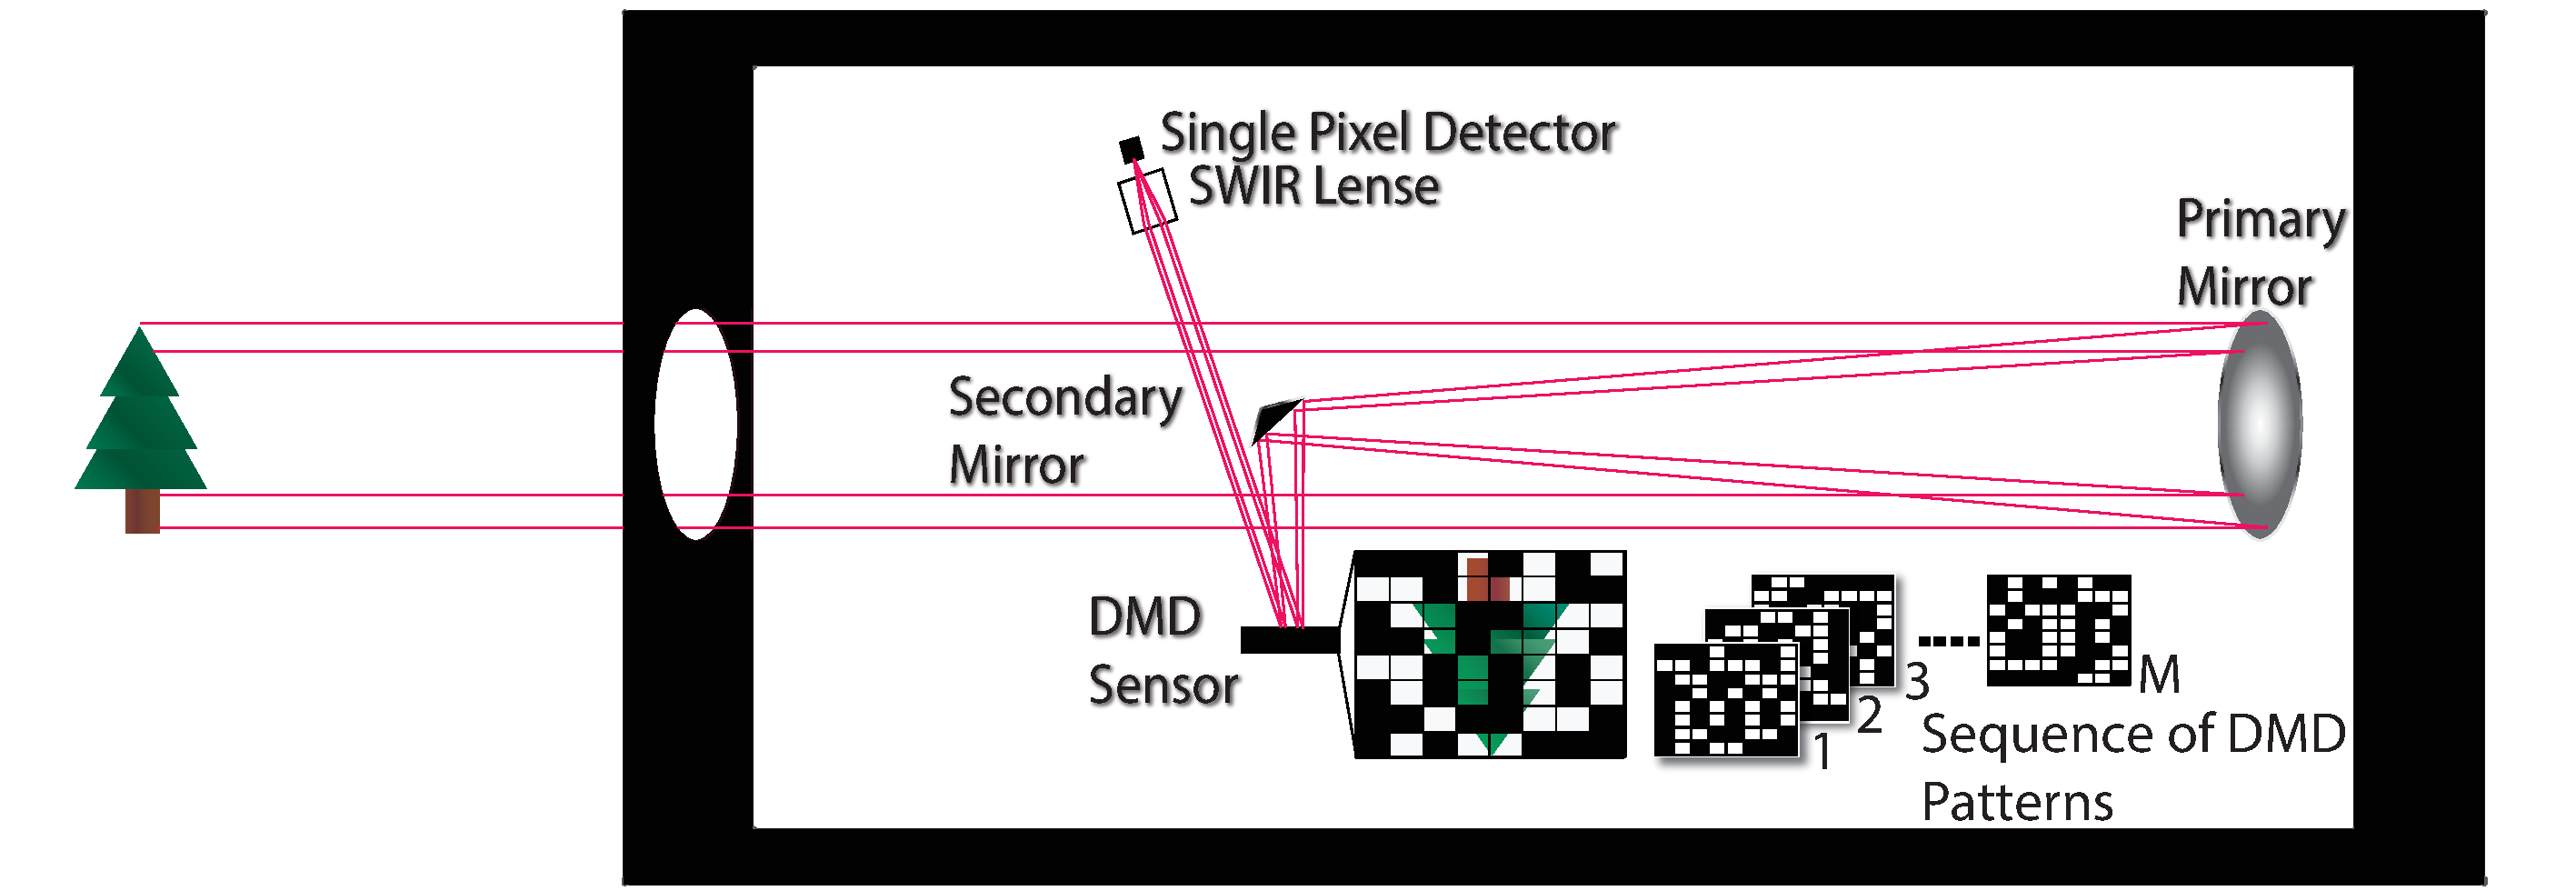
\includegraphics[width = \linewidth]{gfx/System_gif.eps}
	\caption{System overview}
	\label{fig:system_overview}
\end{figure}	

To connect the architecture with the math from CS it can be interpreted as, the light from the scene which is focused on the DMD is the desired signal $\mathbf{x}$, the image. The DMD can individually set each mirror the ether direct the light from each 'pixel' to the single pixel sensor or dump the light i.e a spatial light modulator (SLM). The DMD sets a pattern of pixel of intress which is a measurement matrix $\Phi_m$ to be summarized in the single pixel sensor $y_m$ as a measurement. One measurement is the inner product of a measurement matrix and the signal, $\Phi_m \times x = y_m$. To complete a full measurement the process is repeated with different measurement matrices set on the DMD to the full undetermined linear system $ \mathbf{y} = \mathbf{\Phi}\mathbf{x}$.

\subsection{Measurement matrix \& reconstruction}
How is the measurement matrix chosen? As told before the measurement matrix needs to be incoherent with the sparse transform and the DMD can only direct he light or not which mathematically is ether a zero or a one. The research tells that for example a i.i.d. Gaussian distribution with equal probability of a zero or one will with high probability be incoherent with a natural image scene. But how about the first constraint that the signal $\mathbf{x}$ needs to be sparse or compressible in some basis? Often natural images is not sparse in the spatial domain unless the scene is for example the night sky, well a good property of CS that the scene can be transformed to an other basis like this,

\begin{equation}
\label{eq:CS_1}
\mathbf{y} = \mathbf{\Phi} \mathbf{x} \Leftrightarrow \mathbf{y} = \mathbf{\Phi} \mathbf{\Psi} \mathbf{\Theta},
\end{equation}

where $\mathbf{\Psi}$ is a sparsitfying basis for example to the DCT or Wavelet basis. And $\mathbf{\Theta}$ is the coefficients vector which is more sparse then the spatial coefficent vector $\mathbf{x}$. And the transformation will not comprimize the incoherence between the reconstruction matrix $A = \Psi\Phi$ and the coeficents $\Theta$ in the new basis. This means that the signal $\mathbf{x}$ will be reconstructed with optimization in a more sparse basis $\Theta$ and then transformed back to the spatial domain.\\[0.1in]

What i special about CS is not just how the problem is presented but also how to solve it. It is known that an undetermined linear system as infinite many solution so how does the signal get recovered? CS exploit the characteristics of the signal $x$ which is known to be sparse in some basis. With for example $\ell_1$ optimization,

\begin{equation}
\label{eq:l1_1}
\widehat{\mathbf{\Theta}} = \text{arg min} ||\mathbf{\Theta} ||_{\ell_1} \text{ subject to } \mathbf{\Psi} \mathbf{\Theta} \Theta = y,
\end{equation}    

which means that $\ell_1$ optimization minimizes the non zero elements of $\Theta$ and can exactly reconstruct a K-spares vector or approximate a compressible vector. The exact recovery can be accomplished with high probability using $M \geq \mathcal{O}(K\text{log}(N/K))$ measurements. This is why CS is powerful, it enables sub-Nyquist measurements with exact recovery in the noiseless case which can be approximated in real applications.\\[0.1in]

In the compressed imaging case where noise is present an other optimization algorithm has shown to be more successful at recovering images: total variation. Total variation regularization minimizes the magnitude of the gradient in the image and doing so it preserve edges and piece-wise constant structure in the image which is desired.     

 
\subsection{Motivation}
Why would a SPC be beneficial to a conventional camera? The SPC has more components to work and several measurements have to be made over time while a regular camera measures all pixels on the sensor at the same time and the reconstruction shifts burden to the processor.

\begin{itemize}
\item Why?
\item Compress before the images is taken
\item Cheaper and in some cases only possible case to go to larger resolutions
\item It is more effective then scanning each pixel one by one because the one need to do N samples.
\end{itemize}


\subsection{Aim} 
What image quality can be achieved in natural images captured with a single pixel camera in daylight using state of the art methods?  


\subsection{Research questions} 
\label{sec:RQ}
\begin{itemize}
    \item How can the quality of images reconstructed by CS or a SPC be evaluated?
    \item What is the state of the art method to capture and reconstruct images using a SPC architecture?
    \item What image quality is achieved using state of the art methods applied to the SPC?
\end{itemize}


\subsection{Limitations}
\begin{itemize}
    \item The hardware rig provided by FOI
    \item 
\end{itemize}



\subsection{Thesis outline}

\section{Related work}
\label{sec:related_work}
In this section important, relevant and fundamental articles to this master's thesis is presented each with a summary. The articles covers compressed sensing theory applied to compressed imaging, SPC architecture and how to evaluate the images i.e. the fundamental source of information on how to build a state of the art SPC system and how to evaluate its performance. 

\subsection{Compressive sensing}
\begin{itemize}


\item \cite{book:sm, book:srr} "Sparse Modeling" by G. Y. Grabarnik and  I. Rish and "Sparse and redundant representation" by M Elad is two books which thoroughly presents the topic of sparse and redundant representation and modeling. The fundamental principles and constraints that needs to be fulfilled in CS are described. The books presents different minimization algorithms and how to implement them.   

\item In~\cite{article:CS_donoho1} by "Compressed sensing" David L. Donoho proposed the framework of compressed sensing and the application of images capturing.

\item \cite{article:CS_from_theory_a_sur} "Compressive Sensing: From Theory to Applications, A survey" by S. Qaisar et al. 2013, reviews CS background, theory and mathematics and has a extensive survey of reconstruction algorithm and potential CS applications.

\end{itemize}
\subsection{Compressive imaging}
\begin{itemize}

\item \cite{article:an_Arcitecture_for_CI,article:a_new_ci_arc} "An architechture for compressive imaging" and "A New compressive imaging camera architecture using Optical-Domain Compression" by M. B. Wakin, D Takhar, et al. 2006, presents the first single pixel camera architecture using CS to reconstruct the images. 

\item \cite{article:single_pixel_im_cs} "Single-Pixel Imaging via Compressive Sampling" by M. F. Duarte et al. 2008, is an introduction and summary to CS and CI including the SPC architecture. This article also compares different scanning methodologies and their conditions.   

\item \cite{article:foiSPIS} "Single Pixel SWIR Imaging using Compressed Sensing" by C. Brännlund and D. Gustafsson, 2016, shows the initial results and proof of concept of the SPC architecture at FOI.
  
%\item \cite{article:cs_for_prac_ios_a_tut} "Compressed sensing for practical optical imaging systems: a tutorial"


\item \cite{article:a_high_res_swir} "A high resolution SWIR camera via compressed sensing" is a paper by L. McMackin et al. 2012 at Inview Technology which develop and produces compressive sensing cameras. The paper contains a brief review of CS and CI followed by a presentation of their camera architecture. 

 
\item \cite{mt:EF} "Compressed Sensing for 3D Laser Radar" by E. Fall, 2014, is a master's thesis where CS/CI is evaluated for a potential depth camera architecture using a one pixel sensor.   

\item \cite{article:misuperres} "Multi image super resolution using compressed sensing" by T. Edler et al. 2011, presents the results from using a small detector array instead of just one single sensor, but still using CS to reconstruct the images. With this technique the subsampling ratio and the exposure time is reduced. 

 
	
\end{itemize}
    
\subsection{Measurement matrix \& reconstruction}

\begin{itemize}
    
\item \cite{article:TVAL3} Chengbo Li:s master's thesis "An Efficient Algorithm For Total Variation Regularization with Applications to the Single Pixel Camera and Compressive Sensing" describes a total variation algorithm that Li constructed which solves the CS problem. The algorithm is faster and produces better results for images than previous popular algorithms.   

\item \cite{article:SRM_short, article:SRM_long, article:SRM_block} Fast and Efficient Compressive Sensing Using Structurally Random Matrices (SRM). The articles describes why and how to implement SRM, in these articles the Hadamard or DCT matrices is proposed to replace the random measurement matrix. With SRM the reconstruction time is reduced by replacing matrix multiplication with fast transforms. In addition to improve reconstruction time, the new method does not need to store the measurement matrix in memory, which enables reconstruction of high resolution images. 

\item \cite{article:an_improved_WH_matrix} "An Improved Hadamard Measurement Matrix Based on Walsh Code For Compressive Sensing" shows that sequency-ordered Walsh Hadamard matrix gives better reconstruction than the Hadamard matrix with the same benefits of using the Hadamard matrix. The resulting reconstructed image has near optimal reconstruction performance.
	

\end{itemize}


\subsection{Evaluation}

\begin{itemize}

\item \cite{book:image_processing} "The essential guide to image processing" by Al Boviks contains the majority of fundamental image processing techniques and measurements. Two image quality metrics of interest is PSNR and SSIM which can be used when a reference image is available.
    
\item \cite{article:brisque} "No-Reference Image Quality Assessment
in the Spatial Domain" by M. Anish et al. 2012, is the article describing the blind/referenceless image spatial quality evaluator (BRISQUE). The BRISQUE algorithm evaluates image quality and “naturalness” based on statistics in the image. BRISQUE is used when there is no reference image available and therefore can be used to evaluate images produced by the SPC.  
    
\item \cite{article:FOI_pres_sens} "Prestandamått för sensorsystem" by F. Näsström et al. 2016, describes methods and tools to evaluate sensor systems at FOI. 
    
\end{itemize}



%\subsection{Analysis}



\chapter{Method} \label{sec:method}
In order to answer the research questions stated in section~\ref{sec:RQ}, a state of the art SPC, experiments and evaluation methods needs to be set up. In this section all the necessary hardware and software components and theory will be presented as well as the evaluation techniques. 


\section{Single pixel camera architecture \& hardware}
\label{sec:system}
FOI designed the SWIR SPC platform using a DMD, a Newtonian telescope and a single pixel SWIR detector. The system also has a reference camera in the visual spectrum  which can capture images of the scene reflected on the DMD, check that the patterns are displayed correct on the DMD and simplifying focusing of the image.  

\begin{figure}[H]
    \centering
    \includegraphics[width = 0.9\textwidth]{gfx/SPC.png}
    \caption{The single pixel camera architecture used in this thesis. In the image, the aperture, reflective optics, DMD, reference camera and the single pixel sensor are shown from an areal view including red lines showing the incoming light path.}
    \label{fig:system1}
\end{figure}



As seen in figure~\ref{fig:system1}, light from the scene is focused by the Newtonian telescope and reflected onto the DMD. The mirrors on the DMD can reflect the light individually either into the single pixel sensor or the reference camera. The DMD acts as a Spatial Light Modulator (SLM) and reflects different patterns which is 'summed up' in the single pixel sensor as a voltage intensity. The reconstructed image from the system will have the same resolution as the DMD patterns. The digital light processor (DLP) is the DMD:s control unit which controls which patterns are displayed on the DMD either by reading images from memory or the HDMI video port. 

\subsection{Newtonian telescope}
A Newtonian telescope is a reflecting telescope, using a concave primary mirror and a flat diagonal secondary mirror, see figure~\ref{fig:system1}. In this set-up the telescope act as a lens focusing the scene onto the DMD. The motivation to use a Newtonian telescope instead of a lens system is partly that chromatic aberration is eliminated and partly that a reflective optical system works over a greater range of wavelengths that includes SWIR, near infrared (NIR) and the visible spectrum. This design has a very narrow field of view which give high detailed scenes from a great distance. 


\subsection{DLP and DMD}
The DMD (Texas Instruments DLP4500NIR) is a matrix of micro mirrors that can be individually tilted $\pm 12^{\circ}$ and reflects wavelengths in the range 700-2500 nm. The DMD is controlled by the DLP (DLP\textregistered ~LightCrafter\textsuperscript{TM} 4500) which can be controlled either by video port (HDMI) or by the internal flash memory. The internal memory can theoretically be faster than the video port, but due to constraints in both memory and memory bandwidth, the fastest measurement matrix rate gets stuck at $270 - 300$ Hz. The video port can be operated at 120 Hz and display one bit plane at the time from a $24$ bit signal, which gives a maximum measurement matrix rate $120 \times 24 = 2880$ Hz, but in the current configuration only $60$ Hz frame rate was achieved giving a measurement matrix rate at $1440$ Hz. At this rate with subsampling ratio (the number of measurements relative number of pixels) between $20\% - 30\%$ with $512\times512$ pixel images, the sampling would be acquired in $36 - 52$ seconds. To control the DMD the software "DLP LightCrafter 4500 Control Software" is used.\cite{manual:DLP}\\[0.1in] 

The DMD used in the setup is constructed with a diamond shaped pattern instead of a regular square grid which is used in regular camera image sensors. The diamond shape causes the index of each mirror to be skewed against what a normal grid would look like. As seen in figure~\ref{fig:dmd_index}, the indexes of the mirrors column is two mirror column arrays wide while a row is a single row. 


\begin{figure}[H]
    \centering
    \includegraphics[width = 0.8\textwidth]{gfx/DMD_grid.png}
    \caption{DMD matrix mirror index, left shows each tiles index and right shows the second row and second column in black as set by default from the factory.}
    \label{fig:dmd_index}
\end{figure}

Because the reconstruction algorithm and measurement matrix needs to be a square matrix with the side length with a power of 2, the resulting images ratio would be 2 to 1, while the image should have the ratio 1 to 1. The resulting image would need to be transformed into the real ratio where information potentially gets lost. Therefore the index of mirrors was changed so that each 'pixel' gets two mirrors as seen in figure~\ref{fig:dmd_index2}. This will result in rows and columns gets equal amount of space and the aspect ratio will be preserved 1 to 1. By grouping two mirrors, the amount of light from each "pixel" is doubled and thus should improve the sampled signal quality.

\begin{figure}[H]
    \centering
    \includegraphics[width = 0.8\textwidth]{gfx/DMD_grid2.png}
    \caption{DMD matrix, left shows each tiles index and right shows third row and third column in black.}
    \label{fig:dmd_index2}
\end{figure}

Mathematically the DMD is a binary operator which lets light pass or not, in figure~\ref{fig:dmd_pattern} a typical pattern that could be sent to the DMD is shown.  

\begin{figure}[H]
    \centering
    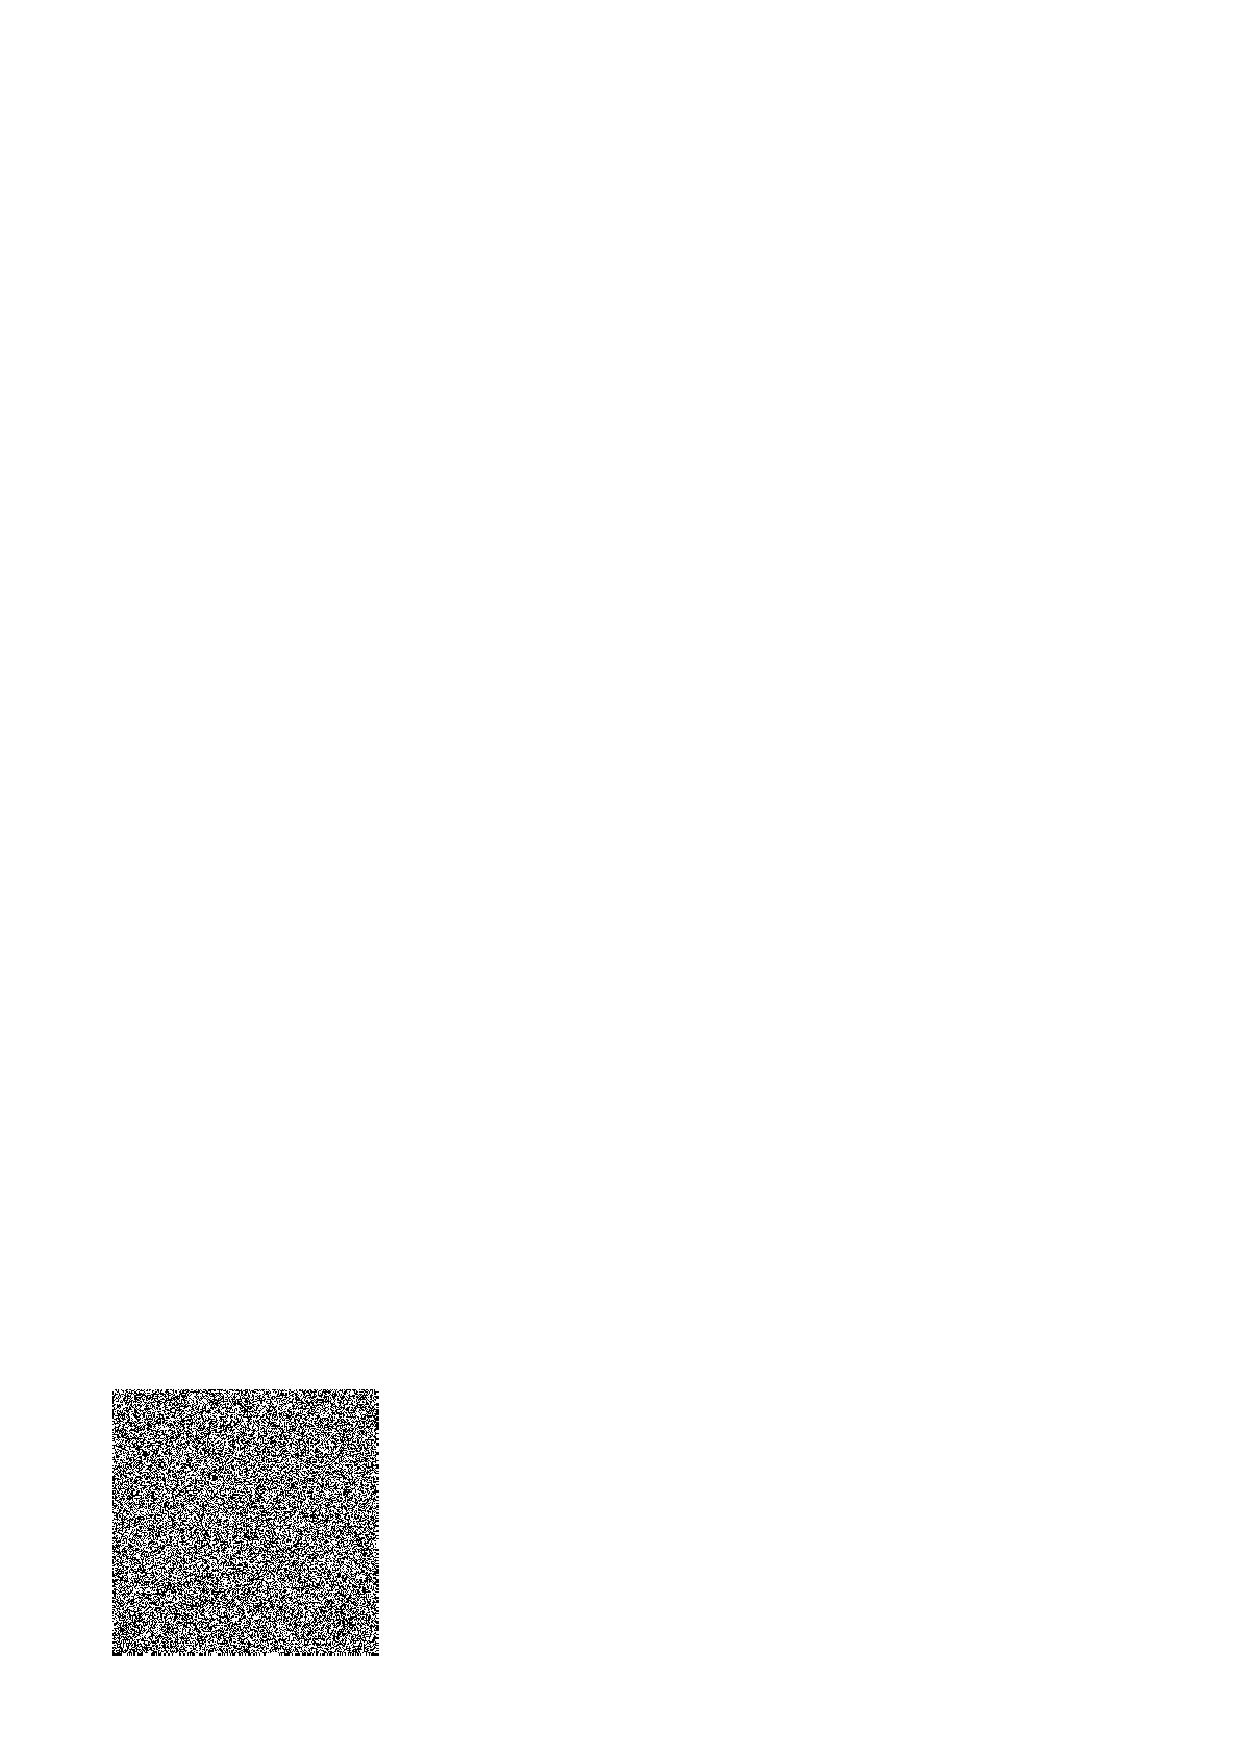
\includegraphics[width = 0.5\textwidth]{gfx/DMD_pattern.png}
    \caption{A typical pseudo random measurement matrix sent to the DMD with the resolution $256 \times 256$ pixels.}
    \label{fig:dmd_pattern}
\end{figure}



\subsection{Lens}
The lens mounted on the single pixel sensor is a 50 mm SWIR Fixed Focal Length Lens with a variable aperture from f-stop f/1.4 designed for wavelengths ranging from 800 nm in the visual spectrum to 2000 nm in the SWIR spectrum. \cite{website:SWIR_objective}

\subsection{Single pixel sensor}
The single pixel sensor is a Thorlabs PDA20C/M and is sensitive in wavelength range 800-1700 nm which is beyond the visual spectrum (390-700 nm). The sensors built-in amplifier outputs an analog signal in volt which the sampler converts to a discrete value. \cite{manual:PDA}

\subsection{Signal spectrum}
All components characteristics assembled, the wavelengths that pass trough the system and measured in the single pixel sensor is between 800-1700 nm.



\section{Compressive imaging}
\label{sec:CI}
Compressive imaging is the name used when sampling and reconstructing images using the compressive sensing method. CI is often realized in form of a SPC but can have different shapes. In this thesis CI is used on the SPC architecture presented in section~\ref{sec:system}. CI exploits the fact that natural images are compressible or approximately sparse in some basis and therefore only a few measurements relative to the image pixel resolution needs to be measured in order to reconstruct the image.\\[0.1in]

CI need to fulfill two constraints in order to utilize CS sampling,  the image needs to be compressible and the complete measurement matrix need to be incoherent with the sparse transform. The first constraint is fulfilled because it is known that natural images are compressible using for example JPEG (using Discrete cosine transform) or JPEG2000 (using wavelet transform) and the second constraint is fulfilled using a measurement matrix with a random characteristic and will be explained further in section~\ref{sec:mm_RIP}.\\[0.1in]
 

The single pixel sensor captures a scene by measuring the light intensity focused onto the detector reflected from the DMD pattern. The DMD pattern changes to obtain new measurements. $M$  measurements are sampled to reconstruct an image with $N$ pixels, where $M \ll N$. Each measurement matrix index is encoded either  by a one or a zero (turning the mirror onto or away from the sensor).\\[0.1in] 

The compressive imaging sampling model is defined as

\begin{equation}
\label{eq:CS1}
   \mathbf{ y = \Phi x + \epsilon}\text{,}
\end{equation}\\[0.1in]


where $\mathbf{x}_{N\times1}$ is the image rearranged as an array with $N$ pixels, $\mathbf{y}_{M\times1}$ is the sampled signal with $M$ measurements, $\mathbf{\Phi}_{M \times N}$ is the complete measurements matrix and $\mathbf{\epsilon}$ is the noise.\\[0.1in] 

In this thesis $\mathbf{\Phi}$ is defined as the \textit{complete measurement matrix} and mainly used in mathematical context, the rows of the complete measurement matrix contains the \textit{measurement matrices}, where one measurement matrix is denoted $\mathbf{\phi}_m$ but can also be denoted as \textit{DMD patterns}. The complete measurement matrix thus contains $M$ measurement matrices.\\[0.1in]


In conventional sampling the number of measurements $M$ needs to be at least equal to the number of pixels $N$ in the image to recover the signal, but CS states that $M$ can be relatively small compared to $N$ given how compressible the image is. This is because the image $\mathbf{x}$ can be represented as  

\begin{equation}
\label{eq:CS2}
   \mathbf{ \Psi \theta = x }\text{,}
\end{equation}\\[0.1in]

where, $\mathbf{\Psi}_{N \times N}$ is some basis matrix and
$\mathbf{\theta}_{N\times1}$ is the coefficients where $\mathbf{\theta}$ is $K$-sparse. $K$-sparse means that the image $\mathbf{x}$ has $K$ non zero elements in basis $\mathbf{\Psi}$, $||\mathbf{\theta}||_0 = K$. Given~(\ref{eq:CS2}), (\ref{eq:CS1}) can be expanded to


\begin{equation}
   \mathbf{ y = \Phi x + \epsilon = \Phi \Psi \theta + \epsilon = A \theta + \epsilon }\text{,}
   \label{eq:CS}
\end{equation}\\[0.1in]

where, $\textbf{A}_{M \times N} = \mathbf{\Phi \Psi}$ is called the reconstruction matrix.\\[0.1in] 

The revelation in~(\ref{eq:CS}) is what makes CS powerful. By sampling the scene using the complete measurement matrix $\mathbf{\Phi}$ (as~(\ref{eq:CS1})) but then in the reconstruction process transforming the complete measurement matrix $\mathbf{\Phi}$ to the reconstruction matrix $\mathbf{A}$ using some basis $\mathbf{\Psi}$, the optimization algorithm can solve the system for the sparse coefficients $\theta$ instead of the spatial image coefficients in $\mathbf{x}$ which are not sparse.\cite{book:sm}\\[0.1in]

A great advantage CI has over regular cameras, where each pixel is sampled separately, is that roughly half the pixels is sampled in one sensor, meaning that background noise of the sensor will be surpassed by the summed intensity of half the pixels making CI very robust to noise.  


\section{Measurement matrix and Restricted isometry property (RIP)}
\label{sec:mm_RIP}
As stated in section~\ref{sec:CI}, the complete measurement matrix needs to be incoherent with the sparse transform. In this section the most powerful constraint on a complete measurement matrix is shown, the restricted isometry property (RIP). \\[0.1in]

In the noiseless case exact recovery of the image $\mathbf{x}$ is achievable if RIP holds for the reconstruction matrix $\mathbf{\Phi} \Rightarrow \mathbf{\Phi\Psi = A}$, the constraint is defined as,

\begin{equation}
    (1-\delta_K)||\mathbf{x}||_{\ell_2}^2\leq||\mathbf{Ax}||_{\ell_2}^2\leq(1+\delta_K)||\mathbf{x}||_{\ell_2}^2 \text{,}
\end{equation}\\[0.1in]

where $\delta_K \in [0.1)$ is the smallest constant to satisfy RIP for a K-sparse signal $\mathbf{x}$. To determine a sampling matrix is a NP-hard problem (which means that there is no feasible way of creating a optimal reconstruction matrix) and generally $\textbf{x}$ is not known and varies, which means that there are no general optimal reconstruction matrices for natural images. Therefore, it is desired to find a general reconstruction matrix that satisfies RIP with high probability. It has been proved that constructing the complete measurement matrix by picking independent and identically distributed (i.i.d.) random variables gives $\delta_K << 1$ with high probability. Constructing the measurement matrices using i.i.d random variables has showed that the number of measurements $M$ needed to satisfy RIP with high probability is $M \geq O(K\text{log}(N/K) \ll N$. \cite{book:srr}\\[0.1in]

The problem of using random matrices is that they need to be stored in memory for the reconstruction algorithm, so when the image resolution is increased the measurement matrix increases exponentially. For images with resolution of $512\times 512$ and larger, the data gets unfeasible for a normal computer to handle.\\[0.1in]  

Fortunately, by changing the complete measurement matrix to structurally random matrices, fast transforms can be used in the reconstruction algorithm instead of vector multiplication, resulting in both faster reconstruction and no need to store the measurement matrix in memory. In this thesis, the permutated sequency ordered Walsh Hadamard measurement matrix (described in section~\ref{sec:SOWHMM}) will be used with the TVAL3 reconstruction algorithm (described in section~\ref{sec:TV}) to achieve higher resolution photos and faster reconstruction.   


\subsection{Permutated sequency ordered Walsh Hadamard measurement matrix}
\label{sec:SOWHMM}
Besides from eliminating the need to store the measuring matrix in computer memory for reconstruction, the permutated sequency ordered Walsh Hadamard matrix (PSOWHM) can be generated when sent to the DMD and thus eliminating the need to store the matrix at all. PSOWHM has approximatly the same characteristics and properties as an i.i.d. random matrix but generally has a higher number of measurements for exact reconstruction of the image, $M \sim (KNs)\log^2(N)$, where $s$ is the average number of non zero indexes in the measurement matrix \cite{lec:fast_CS_SRM}. Research has however shown that there is no significant loss in recovery of the image relative the i.i.d. random measurement matrix~\cite{article:an_improved_WH_matrix}. An other property of PSOWHM is that it only contains -1 and 1, which can easily be converted to 0 and 1 when sent to the DMD. \\[0.1in]


In order to construct the PSOWHM, the fist step is to define the naturally ordered Hadamard matrix and then follow a few additional steps. The naturally ordered Hadamard matrix of dimension $2^k$, $k \in \mathbb{N}$ is constructed by the recursive formula    

\begin{equation}
    H_0 = 1,
\end{equation}

\begin{equation}
    H_1 = \begin{bmatrix}
       1 & 1 \\
       1 & -1\\
     \end{bmatrix},
\end{equation}

and in general,

\begin{equation}
        H_k = \begin{bmatrix}
       H_{k-1} & H_{k-1} \\
       H_{k-1} & -H_{k-1}\\
       \end{bmatrix} = H_1 \otimes H_{k-1}
\end{equation}

where $\otimes$ denotes the Kronecker product.\\[0.1in]

To construct the permutated sequency ordered Walsh Hadamard matrix from the naturally ordered Hadamard matrix these steps are required:

\begin{itemize}
    \item Convert row index $n_H$ to binary.
    \item Convert the binary row index to Gray code.
    \item Apply bit reverse on the Gray code index.
%    \item Remove first row with only ones.
%    \item Permutate columns and choose $M$ rows at random.
\item Order the rows after the bit-reverse to obtain the sequency ordered Walsh Hadamard matrix.
\end{itemize}

The procedure is illustrated with an example in table~\ref{tab:Hadamard_2_Walsh} and equation (\ref{eq:hadamard_2_walsh}).  

\begin{table}[H]
\centering
\begin{tabular}{|r|c|c|c|c|}
\hline
    $n_H$        & 0    & 1     & 2     & 3     \\ \hline
    Binary       & 00   & 01    & 10    & 11    \\ \hline
    Gray code    & 00   & 01    & 11    & 10    \\ \hline
    Bit-reverse  & 00   & 10    & 11    & 01    \\ \hline
    $n_W$        & 0    & 2     & 3     & 1     \\ \hline
    
\end{tabular}
	\caption{Example how to convert a naturally ordered Hadamard matrix to a sequency ordered Walsh Hadamard matrix by shifting row with index $n_W$ to $n_H$.}
	\label{tab:Hadamard_2_Walsh}
\end{table}


\begin{equation}
\label{eq:hadamard_2_walsh}
    H_2 =  \begin{bmatrix}
       1 & 1 & 1 & 1 \\
       1 & -1 & 1 & -1 \\
       1 & 1 & -1 & -1 \\
       1 & -1 & -1 & 1 
       \end{bmatrix} \Rightarrow W_2 = \begin{bmatrix}
       1 & 1 & 1 & 1 \\
       1 & 1 & -1 & -1  \\
       1 & -1 & -1 & 1  \\
       1 & -1 & 1 & -1 
       \end{bmatrix}.
\end{equation}

To use the sequency ordered Walsh Hadamard matrix as a measurement matrix the first row is omitted, permutations to the columns are performed, $M$ rows are choosen at random and the indices with $-1$ shifted to $0$. How the matrix are permutated and which rows are choosen in which order are stored so the reconstruction algorithm can use that information to reverese the process. This method is used to distribute the energy of the signal's sample across all measurements.   \cite{article:SRM_long, article:TVAL3, article:an_improved_WH_matrix}. 


\section{Reconstruction method}
To reconstruct the image $\textbf{x}$, the sparsest set of coefficients in $\theta$ is desired. The optimal approach to find these coefficients would be to use $\ell_0$ minimization


\begin{equation}
   \mathbf{ \hat{\theta}} = \text{arg min } ||\mathbf{\theta}||_0 \text{  subject to  } \mathbf{y = A\theta} \text{.}
\end{equation}\\[0.1in]


This seems simply to be minimizing nonzero indices in $\mathbf{\theta}$ in the sparsifying basis $\mathbf{\Psi}$, but this problem is known to be NP-hard. A better approach is the $\ell_1$ minimization, for example Basis Pursuit denoise (BPDN),

\begin{equation}
    \mathbf{\hat{\theta}} = \text{arg min } ||\mathbf{\theta}||_1 \text{  subject to  } ||\mathbf{y - A\theta}||_2 < \mathbf{\epsilon} \text{.}
\end{equation}\\[0.1in]


In 2006 Donoho~\cite{article:CS_donoho1} for the first time guarantied theoretical $\ell_0\text{/}\ell_1$ equivalence which holds in the CS case, which means using a $\ell_1$ minimizer is guaranteed to find the sparsest solution in polynomial time in the noiseless case which can be approximated in the noisy and compressible signal case. The drawback with the $\ell_1$ minimizer is that it requires more measurements than the optimal case with $\ell_0$ but $M \ll N$ still holds. Since 2006 many more types of optimization algorithms have evolved which solves the problem with different methods but with the same goal: finding the largest, most significant coefficients of $\mathbf{\theta}$. \cite{article:CS_donoho1, article:single_pixel_im_cs, article:a_new_ci_arc}


\subsection{Total variation: TVAL3}
\label{sec:TV}
The reconstruction algorithm that was chosen in this thesis was a total variation (TV) regularization algorithm called TVAL3 and was chosen for its speed and good results in image reconstruction compared to other reconstruction algorithms created for the CS problem \cite{article:TVAL3}. Natural images often contains sharp edges and piecewise smooth areas which the TV regularization algorithm is good at preserving. The main difference between TV and other reconstruction algorithms is that TV considers the gradient of signal to be sparse instead of the signal itself, thus finding the sparsest gradient. 

The TV optimization problem in TVAL3 is defined as  

\begin{equation}
\text{min}_\mathbf{x} \Sigma_i ||D_i \mathbf{x} || \text{, subject to } \mathbf{\Phi x} = 	y \text{, } \mathbf{x} \geq 0 \text{,} 
\label{eq:tval3}
\end{equation}

where $D_i\mathbf{x}$ is the discrete gradient of $\mathbf{x}$ at position $i$.\\[0.1in]

TVAL3 stands for "Total Variation Augmented Lagrangian Alternating Direction Algorithm", where augmented Lagrangian is a method in optimization for solving constrained problems by substituting the original constrained problem with a series of unconstrained subproblems and introducing a penalty term. To solve the new subproblems the alterning direction method is used~\cite{article:TVAL3}.\\[0.1in]

As mentioned earlier in section~\ref{sec:SOWHMM}, the main reason to use the permutated sequency ordered Walsh Hadamard matrix is to eliminate the need to store the matrix in computer memory during reconstruction and to speed up the reconstruction. In TVAL3 there are two multiplications between matrix and a vector that dominates the computation time,

\begin{equation}
\mathbf{\Phi}\mathbf{x}^k \text{ and } \mathbf{\Phi}^\top(\mathbf{\Phi}\mathbf{x}^k-\mathbf{y})\text{.}
\end{equation}

The idea is to replace the multiplication with fast transforms. To explain the concept some observations and new functions need to be defined. The first observation is that the sequency ordered Walsh Hadamard matrix is a transform matrix, which also can be computed with the fast Walsh Hadamard transform (FWHT),

\begin{equation}
\mathbf{W}\mathbf{x} = \text{ FWHT}(\mathbf{x}),
\label{eq:fwht}
\end{equation}

where $W$ is a sequency ordered Walsh Hadamard matrix and $\mathbf{x}$ is the image vector. The Walsh Hadamard transform (WHT) is a generalized class of Fourier transforms, which decomposes the input vector into superposition of Walsh functions.\\[0.1in]

In section~\ref{sec:SOWHMM} it was briefly mentioned in the last paragraph that the measurement matrix columns is permutated and rows are chosen at random to create the measurement matrix from the sequency ordered Walsh Hadamard matrix. To describe the different permutations two functions are defined.\\[0.1in] 

\theoremstyle{definition}
\begin{definition}{Column permutation operator}
$\pi(\cdot)$, permutates the order of the columns in a matrix or a vector from a random seed.
\label{def:col_perm}
\end{definition}

\theoremstyle{definition}
\begin{definition}{Subsampling matrix operator}
$\Pi_M(\cdot)$, chooses $M$ row in a matrix at random and stacks them in a new matrix.
\label{def:subsamp_perm}
\end{definition}


Now the complete measurement matrix $\mathbf{\Phi}$ can be constructed using the sequency ordered Walsh Hadamard matrix, statement in equation~\ref{eq:fwht}, definition~\ref{def:col_perm} and \ref{def:subsamp_perm},


\begin{equation}
\mathbf{\Phi} = \pi(\Pi_M(\mathbf{W})) = \Pi_M(\pi(\mathbf{W}))\text{.}
\end{equation}

Note that it does not matter in which order the functions are applied, it gives the same result. Also note that multiplication between a matrix and a vector where one of the variables has been permuted by $\pi(\cdot)$, the function can change variable without changing the result since,

\begin{equation}
\pi(\mathbf{\Phi})\mathbf{x} = \mathbf{\Phi}\pi(\mathbf{x})\text{.}
\label{eq:pi_trans}
\end{equation}


With all observations combined, the matrix multiplication is replaced with the FWHT and operators in definition~\ref{def:col_perm} and \ref{def:subsamp_perm} as shown in equation~\ref{eq:fwht_def},

\begin{equation}
\mathbf{y} = \mathbf{\Phi}\mathbf{x} = \pi(\Pi_M(\mathbf{W}))\mathbf{x} = \Pi_M(\mathbf{W})\pi(\mathbf{x}) = \Pi_M(\mathbf{W}\pi(\mathbf{x})) = \Pi_M(\text{FWHT}(\pi(\mathbf{x}))\text{.}
\label{eq:fwht_def}
\end{equation}

Using this method will reduce the overall computational complexity considerably and it will make the measurement matrix redundant in the reconstruction. Only the two permutation functions $\pi(\cdot) \text{ and } \Pi_M(\cdot)$ needs to be stored. Eliminating the need for the complete measurement matrix in the reconstruction unlocks the potential to reconstruct images with high resolution ($512\times512$ pixels and larger). \cite{article:SRM_long, article:TVAL3}



\section{Image capturing and processing chain}
\label{sec:image_capturing_and_process_chain}
In figure~\ref{fig:flow_chart} the whole process of capturing an image is presented with all subsystems and signal/image processing steps included.

\begin{figure}[H]
\includegraphics[width = 1\linewidth]{gfx/flowchart3.pdf}
\caption{Block diagram of image capturing and processing chain, from signal acquisition to final image. Each color represents different subsystems in hardware or software (described in section~\ref{sec:p_spc}-\ref{sec:ip}).}
	\label{fig:flow_chart}
\end{figure}

This experimental setup is not a fully automatic system where a button can be pressed and the system produces an image. In the setup the subsystems works completely independently and needs to be operated manually in the right order at the right time. Each color in figure~\ref{fig:flow_chart} represents a subsystem in hardware or software. Each subsystem is described in the following subsections.

 
\subsection{Prepare the SPC}
\label{sec:p_spc}
The first step in the yellow block "Prepare the SPC" (figure~\ref{fig:flow_chart}) is to make sure that the SPC is up and running but also to point the camera at the scene and set the correct focus. The scene is located with the aid of the reference camera (see figure~\ref{fig:system1}), with all the mirrors in the DMD directed to that camera. The focus is adjusted manually by moving the primary mirror back or forth, this procedure may introduce some error to the focus.\\[0.1in]

\subsection{Sampling}
The red blocks subsystem "Start sampling signal from SWIR photo diode" and "Store the raw signal" (figure~\ref{fig:flow_chart}) is conducted in a separate software which controls the A/D converter and thus the sampling. When the SPC is prepared, the sampling of the signal is started with a sampling rate such that every measurement has several sampling points and thus over-samples the signal. The oversampling is needed because when the mirrors move from one pattern to the next, the signal is uncertain for some time. The oversampling is also used to suppress noise from the photo diode (see further section~\ref{sec:signal_process}). After the signal is sampled the obtained signal is stored on the computer manually.

\subsection{Streaming patterns to the DMD}
\label{sec:stream_dmd}
The subsystem "Streaming patterns to the DMD" (figure~\ref{fig:flow_chart}), represented in the purple block, is controlled by two different softwares, one which manipulates the pattern-signal received by the DMD and one which sends the patterns to the DMD. The patterns are sent to the DMD through a HDMI cable where the DMD is set up such that the DMD acts as a second screen to the computer. This enables to show anything on the DMD that the screen can show. The patterns are stored as a video and played back on the DMD "screen" with a media player, which shows each pattern in consecutive order. This is the major bottleneck of the system where each measurement matrix needs to be displayed one after the other depending on how fast frame rate that can be achieved. The naive approach would be to display one pattern per frame which is linked to the frame rate of the DMD. For example, 60 frames per second (fps). For a $512\times 512$ image subsampled at $20\%$ which corresponds to $512\times 512 \times 0.2 = 52429$ patterns which would take $52429/60 = 874 \text{ seconds} = 14.5 \text{ minutes}$ to sample. This is a long exposure time for a still image with the constraint that the scene should be stationary to obtain a stationary signal.\\[0.1in]

Fortunately, with the software "DLP LightCrafter 4500 EVM GUI" controlling the DMD, the received video signal can be manipulated before displayed onto the DMD. The software includes a function which can break down the received 24-bit color image into 1 bit planes which can be displayed in consecutive order. This function improves the naive implementation by a factor of $24$, which reduces the time to sample the image in the given example from $874 \text{ seconds to } 874/24 = 36 \text{ seconds}$. That long exposure time is of course not optimal for natural images outdoors, but acceptable for the experimental setup.\\[0.1in]     


To create the video that feeds the patterns to the DMD each pattern,  i.e. measurement matrix, is created as presented in section~\ref{sec:SOWHMM}. Then each group of 8 unique patterns are stacked in the 8 bit planes of an 8 bit image as seen in figure~\ref{fig:8_to_1_8}.

\begin{figure}[H]
\includegraphics[width = 1\linewidth]{gfx/DMD_12.eps}
\caption{Each group of 8 measurement matrices is stored in separate  bit planes in one 8 bit image.}
	\label{fig:8_to_1_8}
\end{figure}

Then for each group of three 8 bit images a 24 bit color image is constructed as seen in figure~\ref{fig:3_8_to_1_3}. 

\begin{figure}[H]
\includegraphics[width = 1\linewidth]{gfx/DMD_2.eps}
\caption{Each group of three 8 bit images is stored into one 24 bit color image. This is one frame in the video sent to the DMD.}
	\label{fig:3_8_to_1_3}
\end{figure}

The 24 bit color image corresponds to one frame in the video.



\subsection{Signal processing}
\label{sec:signal_process}  
When the sampled signal is stored in the computer the remaining signal/image processing and reconstruction represented by blue blocks in figure~\ref{fig:flow_chart} is conducted in MATLAB. In this section the signal processing of the sampled signal is described.\\[0.1in]

The first step is to refine the raw over-sampled signal so that each measurement matrix corresponds to one measurement in signal $\mathbf{y}$. This is done by first finding every set of indices that correspond to every measurement matrix, see figure~\ref{fig:raw_signal} where the signal indices are isolated by the magenta lines.


\begin{figure}[H]
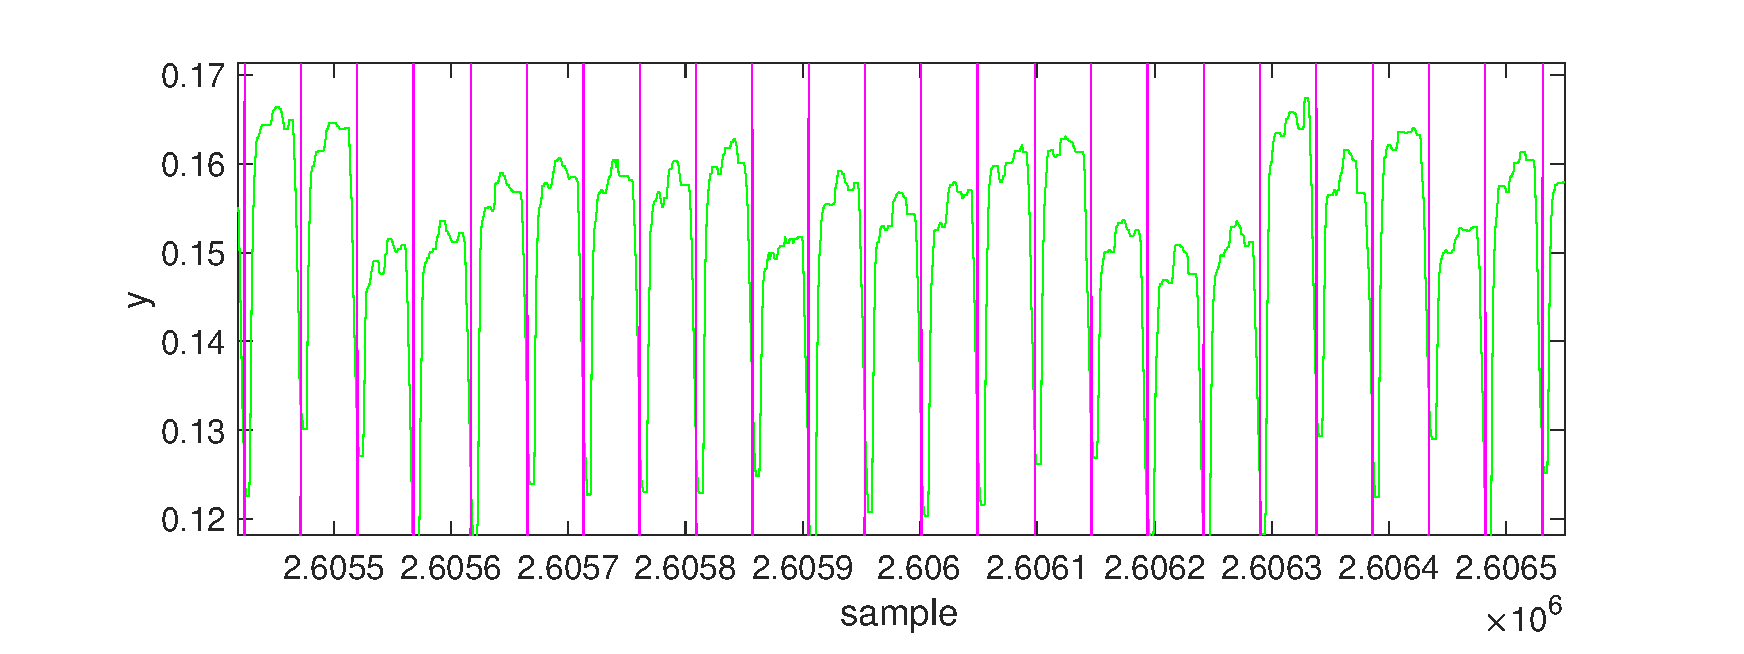
\includegraphics[width = 1\linewidth]{gfx/signal_proc/isolated_raw_signal.eps}
\caption{A simulated noisy over-sampled signal $\mathbf{y}$ where each sample in $\mathbf{y}[m]$ is represented by multiple samples. The magenta lines separating each measurement which corresponds to one measurement matrix.}
	\label{fig:raw_signal}
\end{figure}

The next step is to determine one value for each measurement. This is done in two steps, the first is to omit values which corresponds to the DMD changing pattern close to the magenta lines in figure~\ref{fig:raw_signal}. For the remaining samples, the mean is calculated and set to the value for each sample $\mathbf{y}[m]$, as seen in figure~\ref{fig:detarmain_signal}. 

\begin{figure}[H]
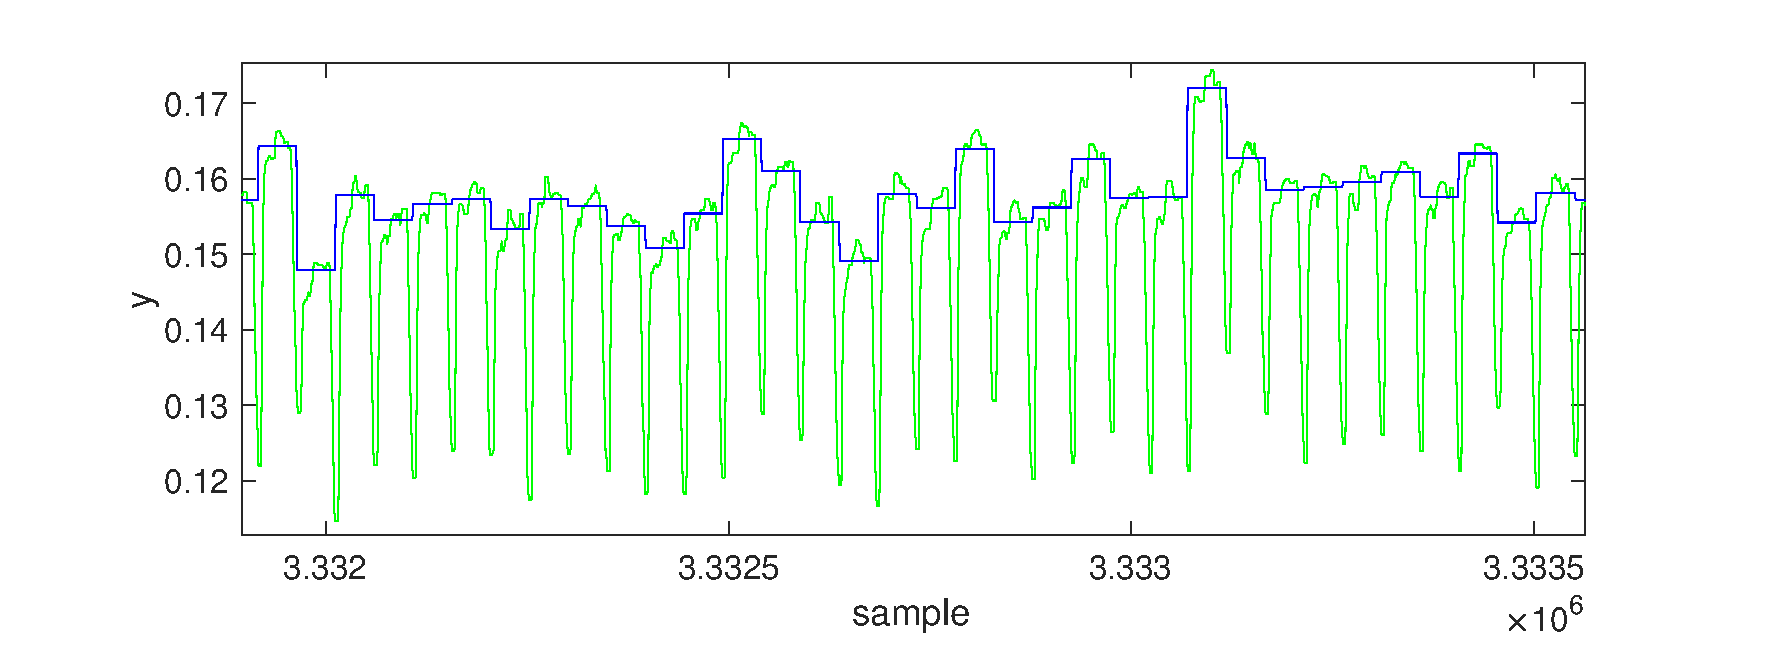
\includegraphics[width = 1\linewidth]{gfx/signal_proc/isolated_final_signal.eps}
\caption{Calculated mean value for each measurement matrix with transition measurements omitted.}
	\label{fig:detarmain_signal}
\end{figure}



\subsection{Dynamics in scene} %: luminance change}
\label{sec:Dynamics_in_scene}
The measured signal $\mathbf{y}$ should be stationary because the image (scene) is assumed to be static. When capturing images outdoors with natural light and long exposure times the image (or every pixel) may not be constant. This ambiguity of each pixel will reduce the reconstruction performance. The potential dynamics in a scene can be divided into two categories, luminance change and object movement. In this subsection the luminance change problem is modeled, and the corresponding algorithm will suppress the impact on the reconstructed image. The object movement problem will not be modeled, but will be avoided by ensuring that the scene is as static as possible.\\[0.1in] 


In natural outdoor images it can be assumed that the primary source of light comes from the sun, but even on a clear day the light intensity from the sun is not constant. If the scene is assumed to be completely stationary, even the slightest intensity change will be amplified by all pixels being measured and thus changing the mean intensity of the measured signal $\mathbf{y}$ which should be stationary. The consequence of the sampled signal $\mathbf{y}$ not being stationary is that reconstruction performance will drop significantly. Therefore a model of light intensity change is created together with an algorithm to restore the signals stationary characteristics.\\[0.1in] 


With the assumption that the scene is constant and the luminance change is uniform over the scene, the problem can be modeled.\\[0.1in]

Start with the original theorem and disregard the noise, 

\begin{equation}
\mathbf{y} = \mathbf{\Phi}\mathbf{x}.
\end{equation}  

The image $\mathbf{x}$ can no be considered constant for all measurements, since the luminance change will change the image $\mathbf{x}$ for every measurement matrix $\mathbf{\phi}_i$. This can be described for one measurement as,  

\begin{equation}
y_i = \mathbf{\phi}_i\mathbf{x}_i = \mathbf{\phi}_i(\mathbf{x} + \mathbf{l}_i) = \mathbf{\phi}_i\mathbf{x} + \mathbf{\phi}_i\mathbf{l}_i ,
\end{equation}
  
where $\mathbf{l}_i$ uniformly adds the same intensity over the whole image $\mathbf{x}$ for measurement $i$. It is known from before that the measurement matrix $\mathbf{\phi}_i$ contains $50\%$ zeros and ones which gives,

\begin{equation}
y_i = \mathbf{\phi}_i\mathbf{x} + \mathbf{\phi}_i\mathbf{l}_i = \mathbf{\phi}_i\mathbf{x} + \frac{N}{2}c_i,
\end{equation}

where $c_i$ is the uniform intensity change coefficient for measurement $i$. This function can be generalized for all measurements,

\begin{equation}
\mathbf{y} =  \mathbf{\Phi}\mathbf{x} + \mathbf{c},
\end{equation}

where $\mathbf{c}$ is the uniform intensity change vector.\\[0.1in]

The goal is to remove the uniform intensity change vector $\mathbf{c}$ from signal $\mathbf{y}$. Using the knowledge that $\mathbf{y}$ should be stationary and assuming that the rate of change in intensity has a much lower frequency than the intensity change between individual measurement matrices, $\mathbf{c}$ can be approximated by the moving mean and removed from $\mathbf{y}$. The moving mean is calculated for each sample $\mathbf{y}[m]$ by calculating the average of $k$ samples centered around $\mathbf{y}[m]$, where $k$ i chosen depending on the DMD pattern rate.\\[0.1in]

Moving mean is defined as

\begin{equation}
\mathbf{y}_{\text{MM}}[m] = \frac{1}{k} \sum_{i = m-\frac{k+1}{2}}^{m + \frac{k+1}{2}} \mathbf{y}[i],
\end{equation}   
		 
where the calculation is made for each sample in $\mathbf{y}$ and thus the algorithm to remove uniform intensity change is,

\begin{equation}
\mathbf{y} = \mathbf{y}_{\text{SAMPLED}} - \mathbf{y}_{\text{MM}} \approx \mathbf{y}_{\text{SAMPLED}} -\mathbf{c}.
\end{equation}

The built in MATLAB function \texttt{movmean} will be used.
		 
%\subsubsection{Dynamics in scene: structure movement}
%Moving objects in the scene is more complex problem than the previous luminance change, both detecting the movement by reading the measured signal and if detected how to remove the problem. In this master's thesis scenes which is known to contain large movement will be avoided, while some small movement for example created by the wind will have to be accepted. In this section a method i proposed to detect a large object rapidly moving in and out of the scene  
%
%In this section a model of a static      

\subsection{Reconstruction}
Reconstruction is performed using the TVAL3 algorithm described in section~\ref{sec:TV}. The algorithm takes the measurement matrix $\mathbf{\Phi}$, the sampled signal $\mathbf{y}$ and the algorithm settings as input arguments and outputs the reconstructed image. The settings used throughout all experments is:

\begin{itemize}
\item \textit{opts.mu} = \texttt{2024}
\item \textit{opts.beta} = \texttt{64}
\item \textit{opts.maxcnt} = \texttt{10}
\item \textit{opts.maxit} = \texttt{1000}
\item \textit{opts.tol\_inn} $= 10^{-5}$
\item \textit{opts.tol} $= 10^{-10}$ 
\item \textit{opts.mu0} = \texttt{16} 
\item \textit{opts.beta0} = \texttt{1}
\item \textit{opts.nonneg} = \texttt{true}
\item \textit{opts.isreal} = \texttt{true}	
\end{itemize} 

This solves for a real non-negative solution as shown in equation~\ref{eq:tval3}. The variables was derived from TVAL3 default image reconstruction settings and then tweaked by changing each variable independently and inspecting the results on a set of test images.


\subsection{Image processing}
\label{sec:ip}
After reconstruction of the image some simple image processing is performed. There are only two operations applied to the reconstructed image and the reason is that the presented image results should represent what can be expected from the system. Furthermore image processing is often applied on special problems or artifacts in the images and it is not desired to cover up if such artifacts exist. Therefore the only two operations used are the median filter and adjusting the intensity for higher contrast.\\[0.1in]

The reconstructed image has a high dynamic range and if only a small set of neighboring pixels are reconstructed with a high intensity peak, which not correlates with the rest of the image, these pixels will drop the contrast in the rest of the image. To remove these peaks the median filter is used. The median filter will also remove "salt and pepper" noise while edges are preserved. The built in MATLAB function \texttt{medfilt2} is used.\\[0.1in]

The second operation is an intensity transform to maximize the contrast in the image, the built in MATLAB function \texttt{imadjust} is used.   


\section{Evaluation: Image quality assessment}
\label{sec:method_eval}
The evaluation will be divided into two categories: reconstructed images from synthetic data and images reconstructed from data acquired by the SPC.\\[0.1in] 

All results are produced with subsampling ratios ranging from 5-30\% and evaluated. The upper limit was set to 30\% partly because of the hardware limitations with long exposure time and partly because the main advantage of CS/CI is to minimize the required subsampling ratio.\\[0.1in]

The evaluation on synthetic data is focused on evaluating the performance of the measurement matrix and reconstruction algorithm. Evaluating synthetic data gives advantages that can not be achieved with images reconstructed using the SPC which is that there is a reference image which the resulting image can be compared to.\\[0.1in]

A reconstructed image from synthetic data is acquired by creating a signal $ \mathbf{ y }_{M\times1}$ taking the inner product of $ \mathbf{y} = \mathbf{\Phi} \mathbf{x} + \epsilon$ where, $\mathbf{x}$ is the synthetic image reshaped to a vector, $\mathbf{\Phi}$ is the measurement matrix with the desired amount of measurements $M$ and synthetic noise $\epsilon$ which can be regulated to simulate different conditions, then using the reconstruction algorithm on the signal $\mathbf{y}$ to obtain the reconstructed image $\mathbf{\hat x}$. Since the measurement matrix and the reconstruction algorithm are independent of the SPC hardware the subsystem can be evaluated independently. Two advantages of evaluating the sensing and reconstruction independently of the SPC is that parameters such as number of measurements and noise can be regulated easy and the second advantage is that a reference image is available for comparison.\\[0.1in] 

\subsection{Evaluation Using reference image}
With a reference image available, two image quality assessments are performed on the result from the simulation: Peak signal-to-noise ratio (PSNR) and structural similarity (SSIM) index. PSNR is defined as

\begin{equation}
    \text{PSNR}[f(x,y),g(x,y)] = 10 \log_{10}\frac{E^2}{\text{MSE}[f(x,y),g(x,y)]}
\end{equation}
 
where, $f(x,y)$ and $g(x,y)$ are the intensity in pixel $(x,y)$, $E$ is the maximum possible pixel value and MSE is the mean square error between the images defined as

\begin{equation}
\text{MSE}[f(x,y),g(x,y)] = \frac{1}{mn}\sum_{x=0}^{m-1}\sum_{y=0}^{n-1}[f(x,y) - g(x,y)]^2.
\end{equation}

The SSIM algorithm is not focused on pixel to pixel differences like PSNR, but instead of the structure of the image in small windows. SSIM separates  luminance, contrast and structure and calculates the difference in each category in a small window to calculate the similarity of the images. The SSIM index is defined as

\begin{equation}
\text{SSIM}[f(x,y),g(x,y)] = \sum_nl[f(n),g(n)]^\alpha c[f(n),g(n)]^\beta s[f(n),g(n)]^\gamma ,
\end{equation}

where $n$ is the window, $\alpha=\beta=\gamma = 1$ and 

\begin{equation}
\displaystyle \text{luminance: } l = \frac{2\mu_{f(n)}\mu_{g(n)} + C_1}{\mu_{f(n)}^2 + \mu_{g(n)}^2 + C_1},
\end{equation}
\begin{equation}
\text{contrast: } c = \frac{2\sigma_{f(n)}\sigma_{g(n)} + C_2}{\sigma_{f(n)}^2 + \sigma_{g(n)}^2 + C_2},
\end{equation}
\begin{equation}
\text{structure: } s = \frac{\sigma_{f(n)g(n)} + C_3}{\sigma_{f(n)} \sigma_{g(n)} + C_3},
\end{equation}

where,

\begin{itemize}
\item $\mu_{f(n)}$ and $\mu_{g(n)}$ is window mean.
\item $\sigma_{f(n)}$ and $\sigma_{g(n)}$ is window standard deviation.
\item $\sigma_{f(n)g(n)}$ is window cross covariance.
\item $C_1 = 0.01*255$, (MATLAB default).
\item $C_2 = 0.03*255$, (MATLAB default).
\item $C_1 = C_2/2$, (MATLAB default).
\end{itemize} 

Which summarizes to

\begin{equation}
\text{SSIM}[f(x,y),g(x,y)] = \sum_n \frac{(2\mu_{f(n)}\mu_{g(n)} + C_1)(2\sigma_{f(n)g(n)} + C_2)}{(\mu_{f(n)}^2 + \mu_{g(n)}^2 + C_1)(\sigma_{f(n)}^2 + \sigma_{g(n)}^2 + C_2)}.
\end{equation} 

The SSIM index has a max value of 1 when the images are identical which makes it easy to read. \cite{book:image_processing}

\subsection{Evaluation Using no reference quality assessment}
In order to evaluate image quality when there is no reference image to compare against, the BRISQUE algorithm is used as a complement. BRISQUE is a no reference image quality assessment model which is based on natural scene statistics and quantifies the "naturalness" of the image.    \cite{article:brisque}

\subsection{Evaluating Using Edge response}
\label{sec:edge_res_def_method}
The edge response measures the sharpness of the image by calculating the distance in pixels required for an edge in the image to rise. In this master's thesis, the distance required for the edge response to rise from 10\% to 90\% was chosen, see figure~\ref{fig:edge_response_def}. This evaluation is performed on static images captured in constant light indoors for consistent results. Furthermore, the motive of the image is slanted geometric objects printed on a sheet of paper.\cite{article:FOI_pres_sens}
 
\begin{figure}[H]
\includegraphics[width = 1\textwidth]{./result/edge_response.eps}
	\caption{Definition of 10-90\% Edge response.}
	\label{fig:edge_response_def}
\end{figure}





\section{Method criticism}
\begin{itemize}
    \item The BRISQUE algorith is not designed for SWIR images or SPC:s characteristics noise. Therefore the results may not reflect how the quality assessment would answer to visual wavelength cameras. BRISQUE definition of "naturalness" may not reflect the images captured by the SPC. 
    \item The effect on the reconstructed images caused by the DMD mirrors alignment and pairing is not known.
\end{itemize}
%LSE - absolute error but does not say much about how humans perceives the image.\\


\section{Evaluation}
\label{sec:Evaluation}
This section is structured as, for each experiment and setup a detailed explanation and motivation on how and why the experiment is needed followed by the results of that experiment. The experiments are motivated by gathering as much information and results as possible to answer the research questions. The first subsection~\ref{sec:SD} will present the results from experiments with synthetic data where a reference image is available. The second subsection~\ref{sec:eval_spc} will present the result from images reconstructed from the SPC. No perfect reference image is available in those experiments therefore the images will be evaluated against near optimal image, no reference QA and against a state of the art SWIR camera. 



\subsection{Synthetic data}
\label{sec:SD}

\subsubsection{PSNR, SNR, SSIM}

\begin{figure}[H]
    \centering
    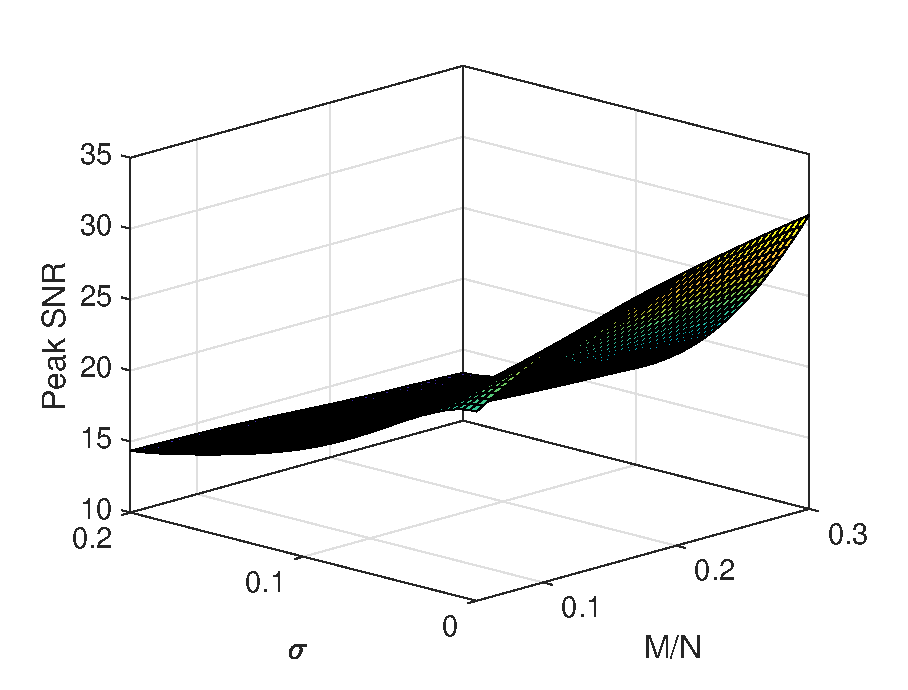
\includegraphics[width = 0.7\linewidth]{result/synt_sss/PSNR_fit.eps}
    \caption{Peak SNR result depending on number of measurements and simulated noise level.}
    \label{fig:psnr_3d}
\end{figure}

\begin{figure}[H]
    \centering
    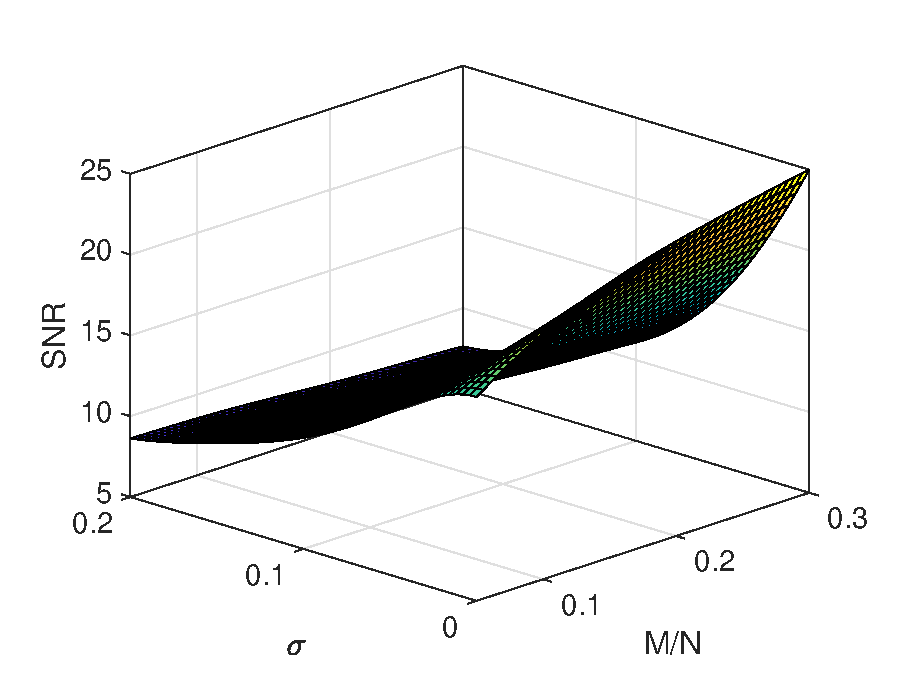
\includegraphics[width = 0.7\linewidth]{result/synt_sss/SNR_fit.eps}
    \caption{SNR result depending on number of measurements and simulated noise level.}
    \label{fig:snr_3d}
\end{figure}

\begin{figure}[H]
    \centering
    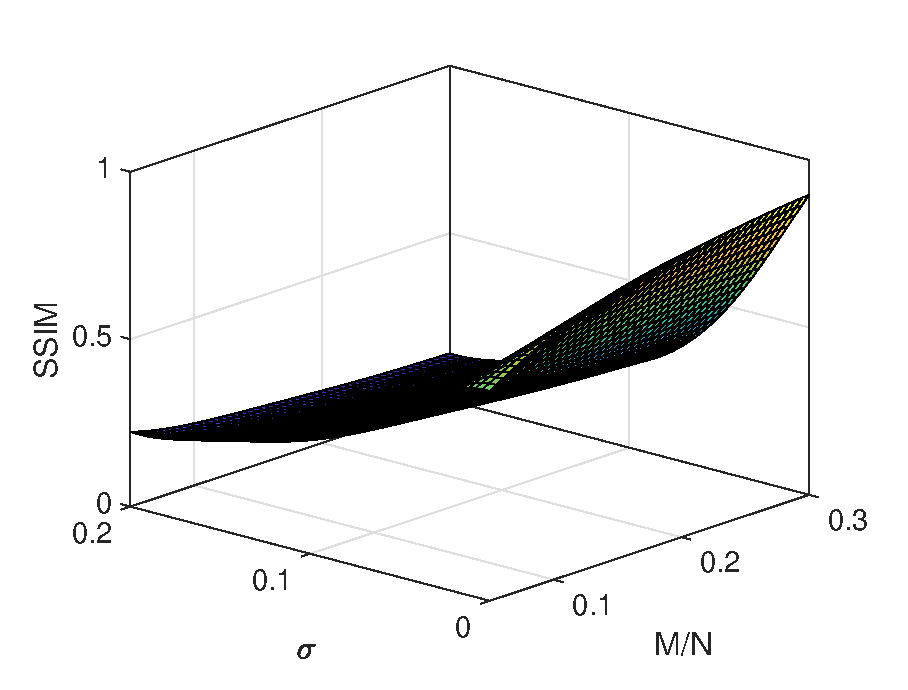
\includegraphics[width = 0.7\linewidth]{result/synt_sss/SSIM_fit.eps}
    \caption{SSIM result depending on number of measurements and simulated noise level.}
    \label{fig:snr_3d}
\end{figure}

\subsubsection{No Reference quality assessment}
BRISQUE lower score is better.

\begin{figure}[H]
    \centering
    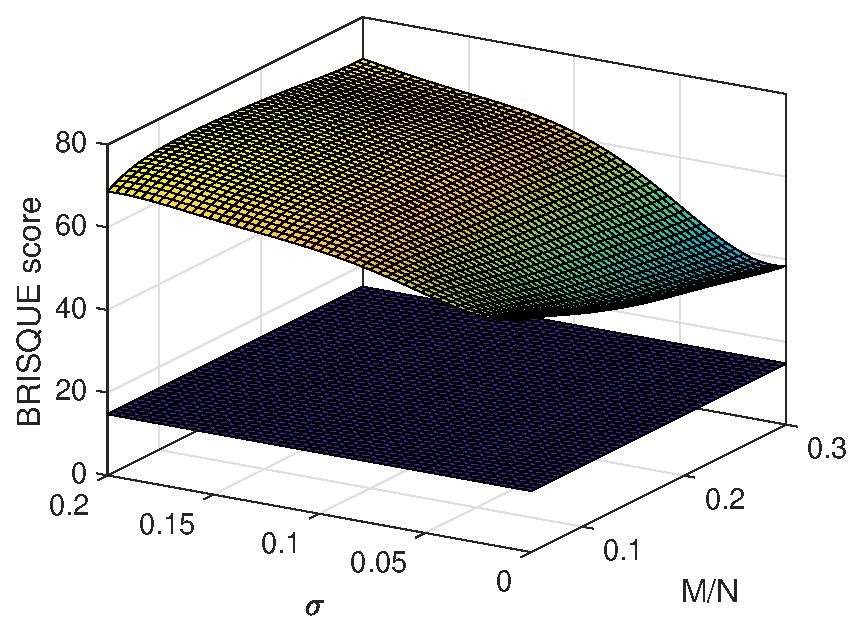
\includegraphics[width = 0.7\linewidth]{result/synt_brisque/BRISQUE_fit.eps}
    \caption{BRISQUE result depending on number of measurements and simulated noise level. Lower surface is reference image score.}
    \label{fig:Brisque_3d}
\end{figure}

\begin{figure}[H]
    \centering
    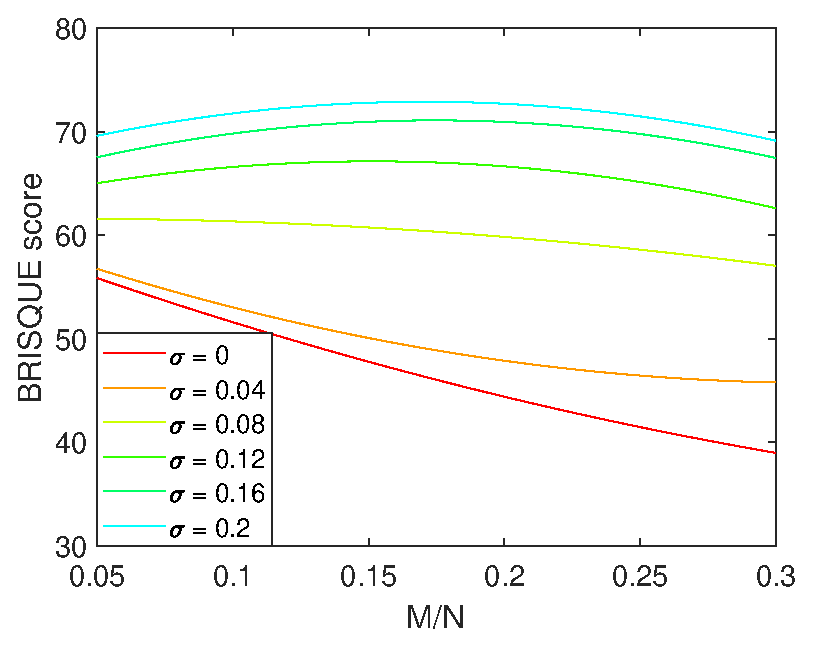
\includegraphics[width = 0.7\linewidth]{result/synt_brisque/Brisque_fit_flat.eps}
    \caption{BRISQUE result depending on number of measurements for different simulated noise levels.}
    \label{fig:Brisque_2d}
\end{figure}



\subsubsection{Dynamics in scene}
Dynamics in the scene can roughly be divided into three separate scenarios, in this section each of them will tested in a controlled environment with each scenario isolated to show how the signal and the reconstructed image is effected.\\[0.1in]

In the first scenario a object will be placed in an image but for each measurement matrix the location of the object will be moved in a bounded area of the image. This will model as a scene where the background is static but a person is standing in the same spot but moving around.

\begin{figure}[H]
    \centering
\begin{minipage}[t]{0.32\textwidth}
    \includegraphics[width=1\textwidth]{result/dynamic/local/local_whole_time_org.png}
    \subcaption{Original reference image}
    \label{fig:local_1}
\end{minipage}
\begin{minipage}[t]{0.32\textwidth}
    \includegraphics[width = \textwidth]{result/dynamic/local/local_whole_time_ref.png}
    \subcaption{Reconstructed $30\%$ image from reference image without movement}
    \label{fig:local_2}
\end{minipage}
\begin{minipage}[t]{0.32\textwidth}
    \includegraphics[width = \textwidth]{result/dynamic/local/local_whole_time_res_psnr_29_snr_25_sssim_91.png}
    \subcaption{Reconstructed $30\%$ image with local movement}
    \label{fig:local_3}
\end{minipage}
    \caption{Local movement}
    \label{fig:local_dyn}
\end{figure}

The difference between figure~\ref{fig:local_2} and \ref{fig:local_3} is visible with the naked eye, not only does the object moving around get blurry and noisy but the whole image globally. In table~\ref{tab:local_dyn}...

\begin{table}[H]
    \centering
  \begin{tabular}{ | l | l | l |}
    \hline
    Peak SNR & SNR & SSIM \\ \hline
    29 & 25 & 91 \\ 
    \hline
  \end{tabular}
      \caption{Effects comparing non perturbed reconstructed image against reconstructed image with local movement}
    \label{tab:local_dyn}
\end{table}

Commenting the result from the table... In figure~\ref{fig:local_signal} the effects of the movement is shown plotted against the non perturbed signal.\\[0.1in]

\begin{figure}[H]
    \centering
\begin{minipage}[t]{0.495\textwidth}
    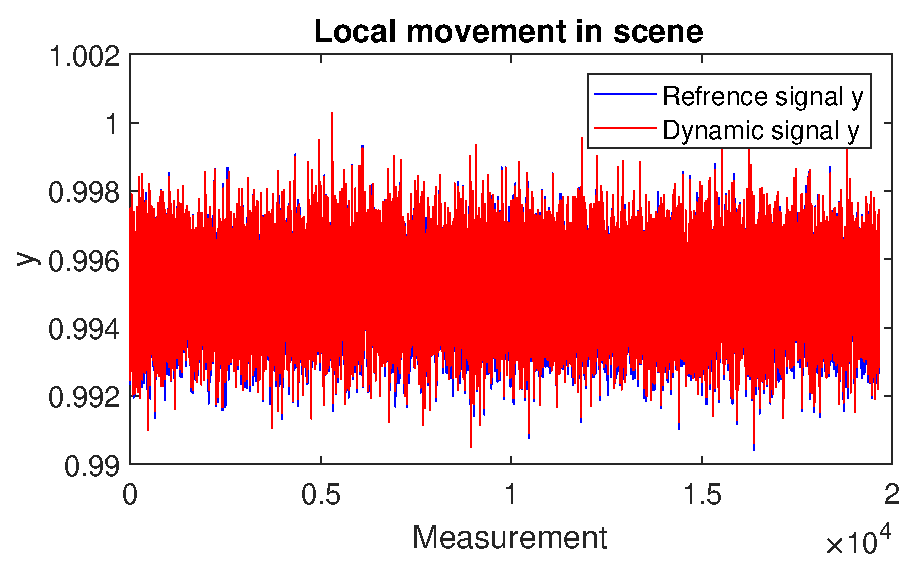
\includegraphics[width=1\textwidth]{result/dynamic/local/local_whole_time.eps}
    \subcaption{Signal.}
    \label{fig:local_sig_1}
\end{minipage}
\begin{minipage}[t]{0.495\textwidth}
    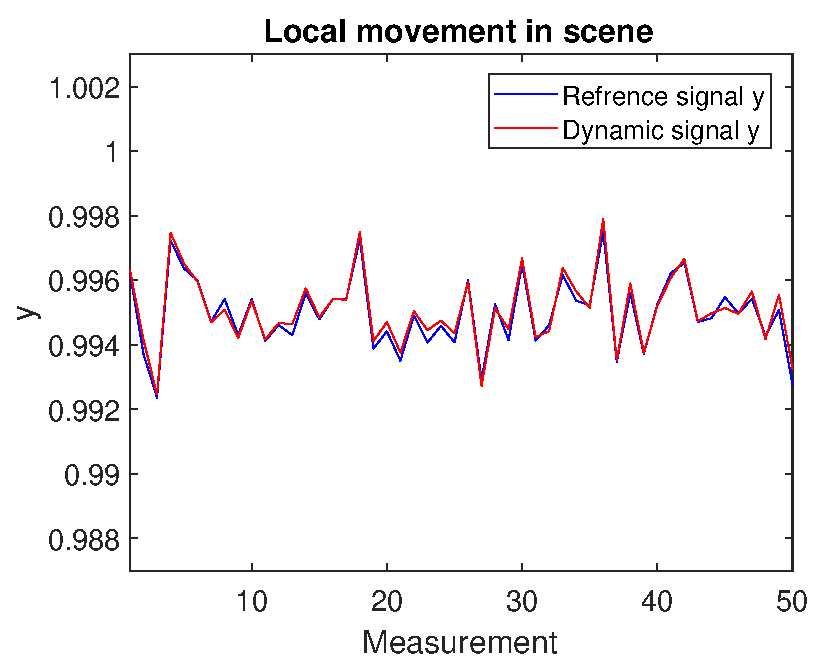
\includegraphics[width = \textwidth]{result/dynamic/local/local_whole_time_win.eps}
    \subcaption{Zoomed in view of the signal.}
    \label{fig:local_sig_2}
\end{minipage}
    \caption{Local movement, acquired signal}
    \label{fig:local_sig}
\end{figure}


As seen in figure~\ref{fig:local_sig_1} there is no obvious difference between the non perturbed reference signal and the distorted signal. In figure~\ref{fig:local_2} where some of the samples is displayed no large difference can be seen ether, the conclusion of this test implies that local movement in a scene will cause noise in the image globally and especially locally where the movement occurred. It also implies that local movement is very hard to detect on the signal even if a reference signal is available.\\[0.1in] 

%%%%%%%%%% Second scenario %%%%%%%%%%%%%%%%

The second scenario is an object is passing through, moves out or moves to an other place in the scene far from the original place. In other words, large global movement in the scene. The problem is modeled with a static background then as the simulated measurement is acquired the same object as in the first experiment will cross the scene, like a car,human or animal might do when using the SPC. The object will cross the scene in 1000 measurements of approximately 19000, corresponding to approximately $0.7$ seconds when capturing with the SPC in its current setup.



\begin{figure}[H]
    \centering
\begin{minipage}[t]{0.32\textwidth}
    \includegraphics[width=1\textwidth]{result/dynamic/fly/flyby_1sec_org.png}
    \subcaption{Original reference image}
    \label{fig:fly_1}
\end{minipage}
\begin{minipage}[t]{0.32\textwidth}
    \includegraphics[width = \textwidth]{result/dynamic/fly/flyby_1sec_ref.png}
    \subcaption{Reconstructed $30\%$ image from reference image without movement}
    \label{fig:fly_2}
\end{minipage}
\begin{minipage}[t]{0.32\textwidth}
    \includegraphics[width = \textwidth]{result/dynamic/fly/flyby_1sec_res_psnr_23_snr_18_sssim_58.png}
    \subcaption{Reconstructed $30\%$ image with object passing trough}
    \label{fig:fly_3}
\end{minipage}
    \caption{Object passing trough scene.}
    \label{fig:fly_dyn}
\end{figure}

The difference between figure~\ref{fig:fly_2} and \ref{fig:fly_3} is visible with the naked eye, A global noise arises in the image and the object cant be seen. In table~\ref{tab:fly_dyn}...


\begin{table}[H]
    \centering
  \begin{tabular}{ | l | l | l |}
    \hline
    Peak SNR & SNR & SSIM \\ \hline
    23 & 18 & 58 \\ 
    \hline
  \end{tabular}
      \caption{Effects comparing non perturbed reconstructed image against reconstructed image with local movement}
    \label{tab:fly_dyn}
\end{table}


Commenting the result from the table... In figure~\ref{fig:fly_signal} the effects of the movement is shown plotted against the non perturbed signal.\\[0.1in]


\begin{figure}[H]
    \centering
\begin{minipage}[t]{0.495\textwidth}
    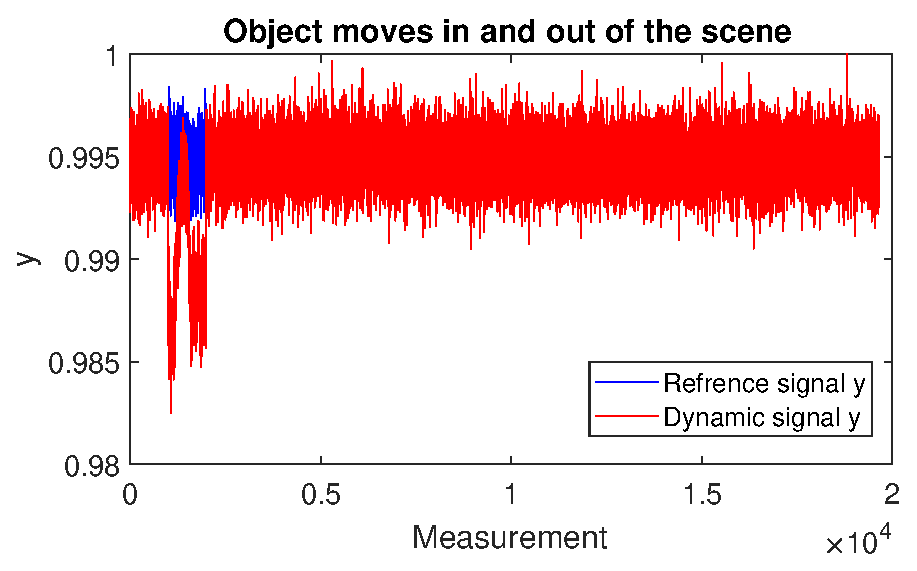
\includegraphics[width=1\textwidth]{result/dynamic/fly/flyby_sig.eps}
    \subcaption{Signal.}
    \label{fig:local_sig_1}
\end{minipage}
\begin{minipage}[t]{0.495\textwidth}
    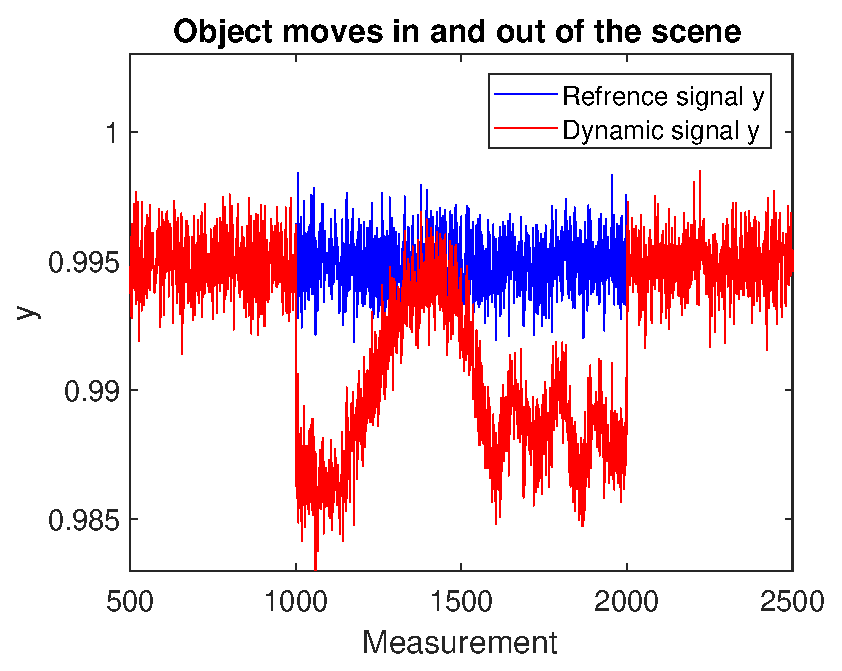
\includegraphics[width = \textwidth]{result/dynamic/fly/flyby_plot_win.eps}
    \subcaption{Zoomed in view of the signal.}
    \label{fig:local_sig_2}
\end{minipage}
    \caption{Global movement, acquired signal}
    \label{fig:local_sig}
\end{figure}

\begin{itemize}
    \item Large changes in the scene can be detected
    \item Remove the identified measurements to get a good signal 
\end{itemize}

%%%%%%%%%%%% Third %%%%%%%%%%%%%%%

The third scenario i luminance change in the scene caused by clouds occludes the sun or the light intensity from the lights is not constant. This scenario is modeled by adding or subtracting the global intensity in the image over the measurements. 

\begin{figure}[H]
    \centering
\begin{minipage}[t]{0.245\textwidth}
    \includegraphics[width=1\textwidth]{result/dynamic/lum/intense_change_org.png}
    \subcaption{Original reference image}
    \label{fig:lum_1}
\end{minipage}
\begin{minipage}[t]{0.245\textwidth}
    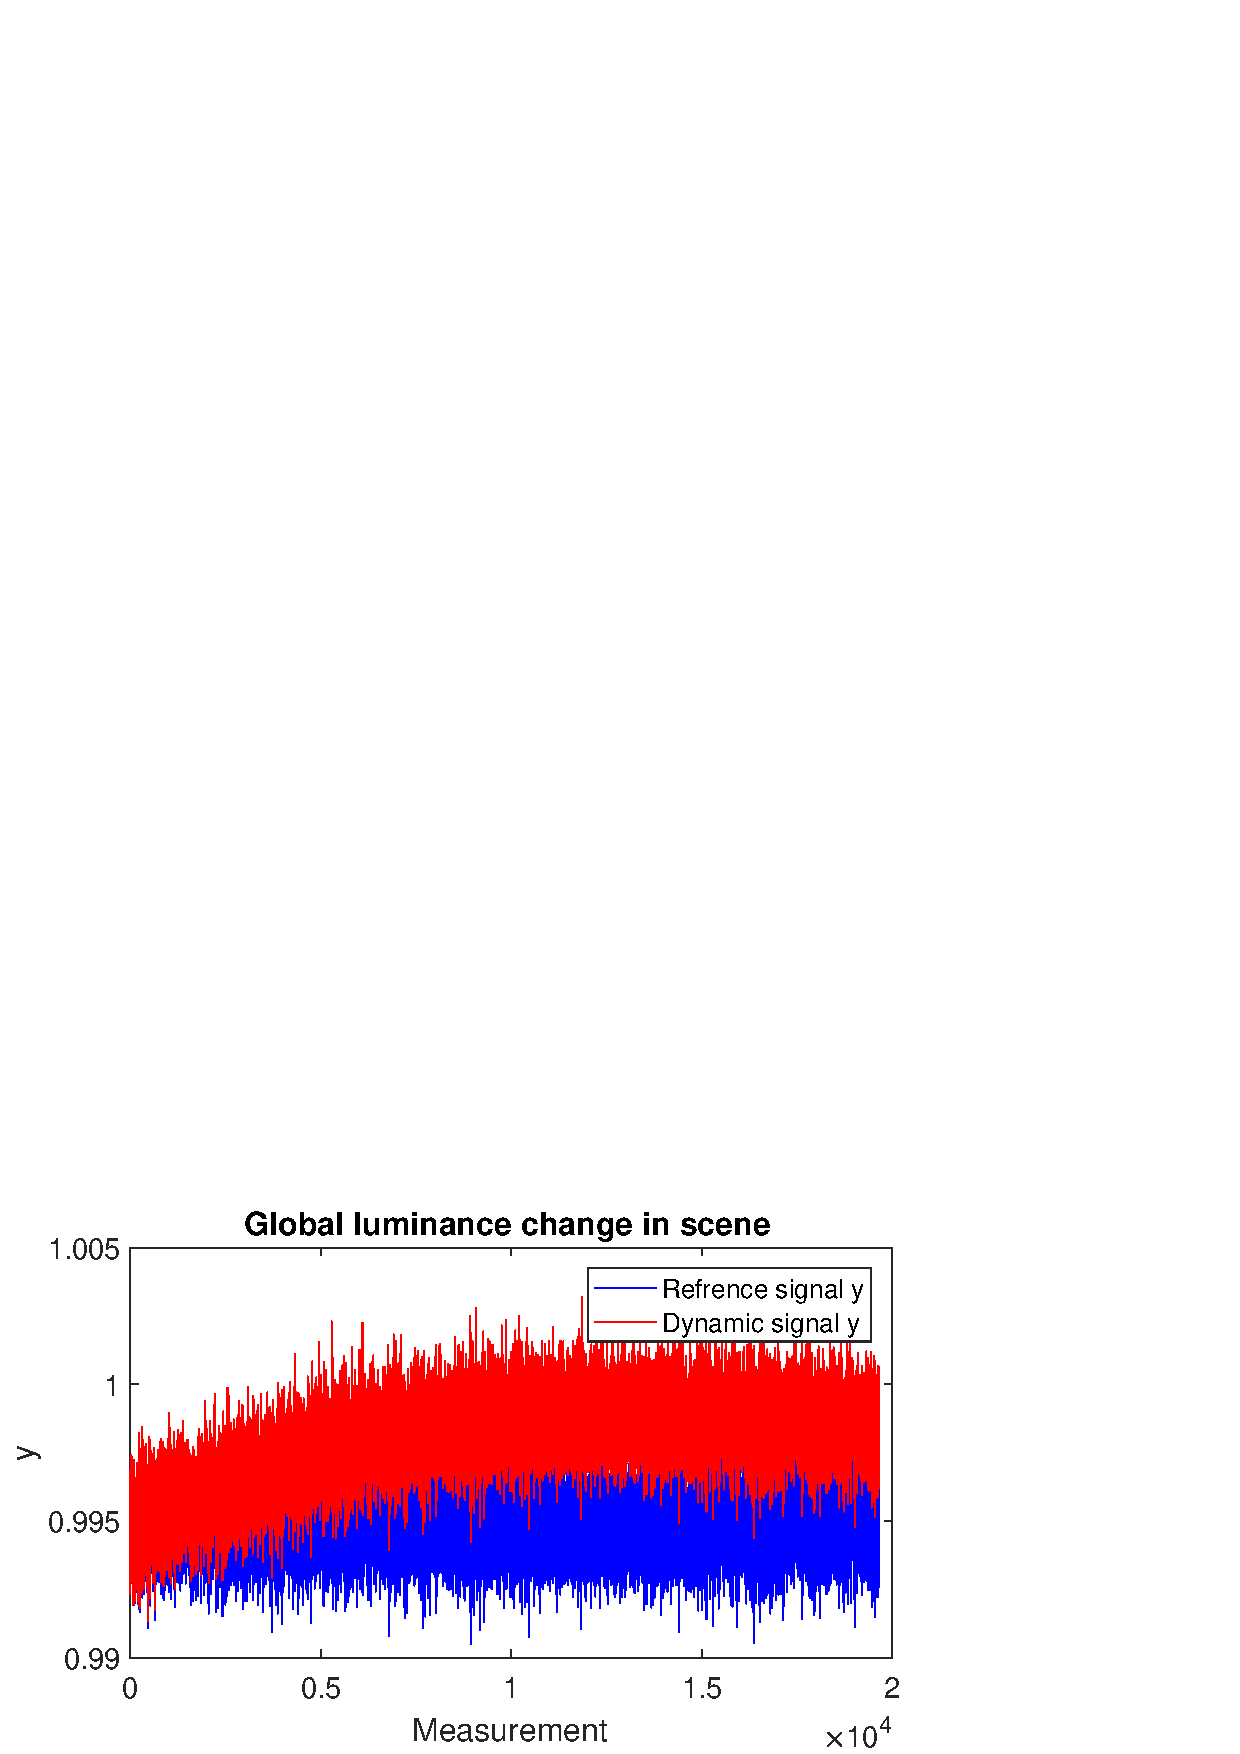
\includegraphics[width = \textwidth]{result/dynamic/lum/intense_change.png}
    \subcaption{Reconstructed $30\%$ image from reference image without movement}
    \label{fig:lum_2}
\end{minipage}
\begin{minipage}[t]{0.245\textwidth}
    \includegraphics[width = \textwidth]{result/dynamic/lum/intense_change_psnr_19_snr_14_sssim_38.png}
    \subcaption{Reconstructed $30\%$ image with global luminance change}
    \label{fig:lum_3}
\end{minipage}
\begin{minipage}[t]{0.245\textwidth}
    \includegraphics[width = \textwidth]{result/dynamic/lum/intense_change_movemean_psnr_33_snr_29_sssim_93.png}
    \subcaption{Reconstructed $30\%$ image with mean subtraction}
    \label{fig:lum_4}
\end{minipage}
    \caption{Global luminance change in scene.}
    \label{fig:lum_dyn}
\end{figure}


The difference between figure~\ref{fig:lum_2} and \ref{fig:lum_3} is visible with the naked eye, A global noise arises in the image, but as seen in figure~\ref{fig:lum_4} the effect can be suppressed explained under figure~\ref{fig:lum_sig}. In table~\ref{tab:fly_dyn}...


\begin{table}[H]
    \centering
  \begin{tabular}{ | l | l | l | l |}
    \hline
     & Peak SNR & SNR & SSIM \\ \hline
    Perturbed signal & 19 & 14 & 38 \\ \hline
    Mean subtracted signal & 33 & 29 & 93 \\
    \hline
  \end{tabular}
      \caption{Effects comparing non perturbed reconstructed image against reconstructed image with global luminance change}
    \label{tab:lum_dyn}
\end{table}


Commenting the result from the table... In figure~\ref{fig:lum_signal} the effects of global luminance is shown plotted against the non perturbed signal.\\[0.1in]


\begin{figure}[H]
    \centering
\begin{minipage}[t]{0.495\textwidth}
    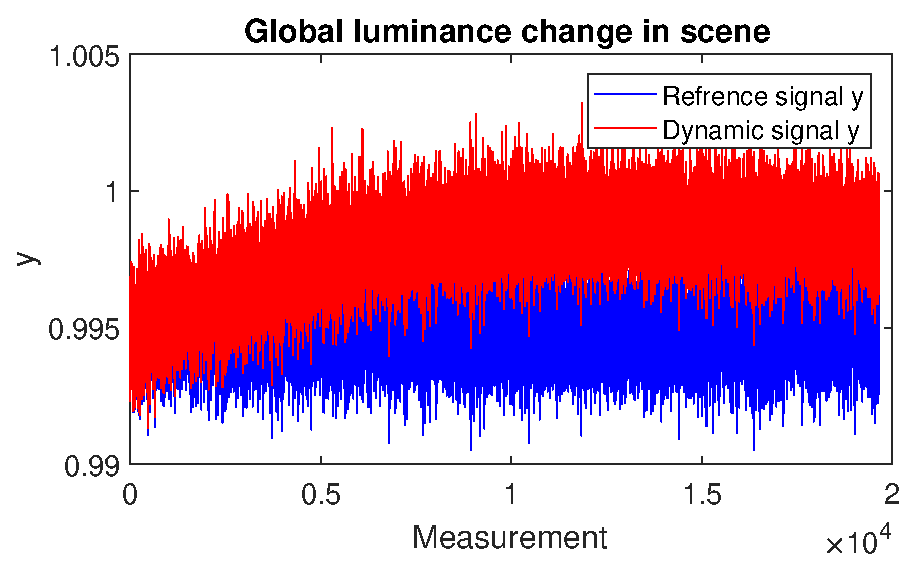
\includegraphics[width=1\textwidth]{result/dynamic/lum/intense_change.eps}
    \subcaption{Signal.}
    \label{fig:lum_sig_1}
\end{minipage}
\begin{minipage}[t]{0.495\textwidth}
    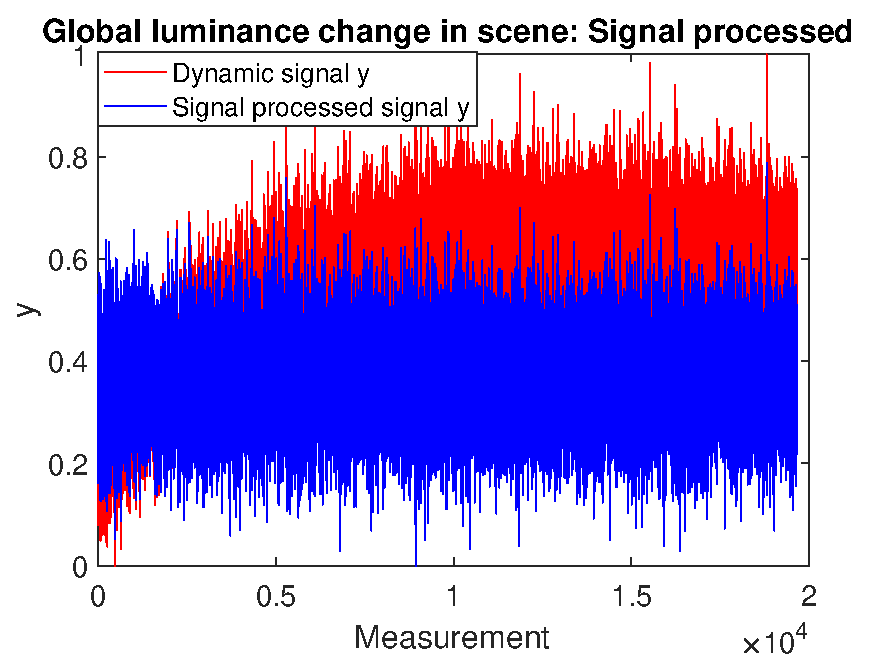
\includegraphics[width = \textwidth]{result/dynamic/lum/intense_change_sp.eps}
    \subcaption{Zoomed in view of the signal.}
    \label{fig:lum_sig_2}
\end{minipage}
\begin{minipage}[t]{0.495\textwidth}
    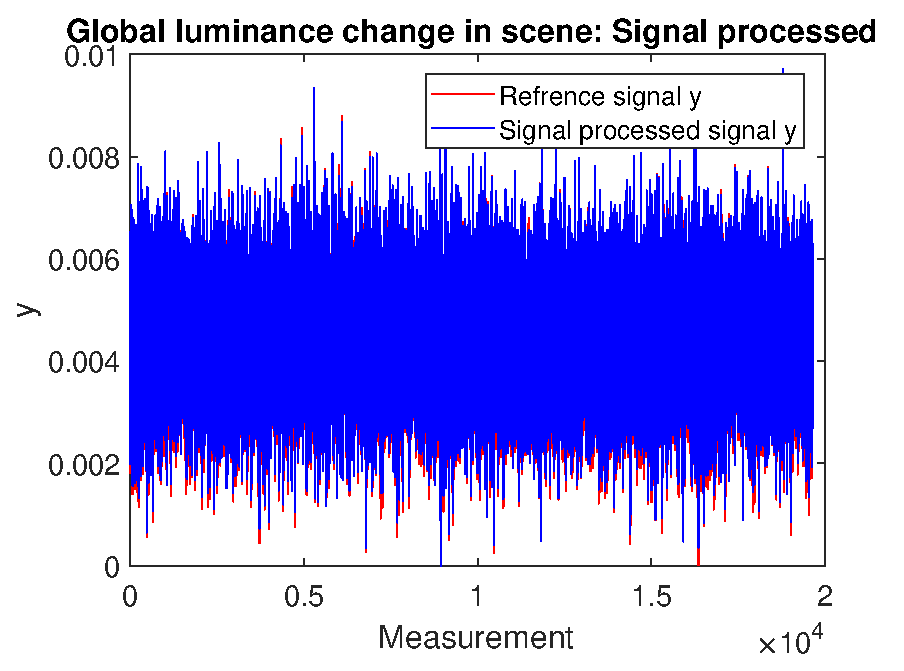
\includegraphics[width=1\textwidth]{result/dynamic/lum/intense_change_sp_ref.eps}
    \subcaption{Signal.}
    \label{fig:lum_sig_3}
\end{minipage}
\begin{minipage}[t]{0.495\textwidth}
    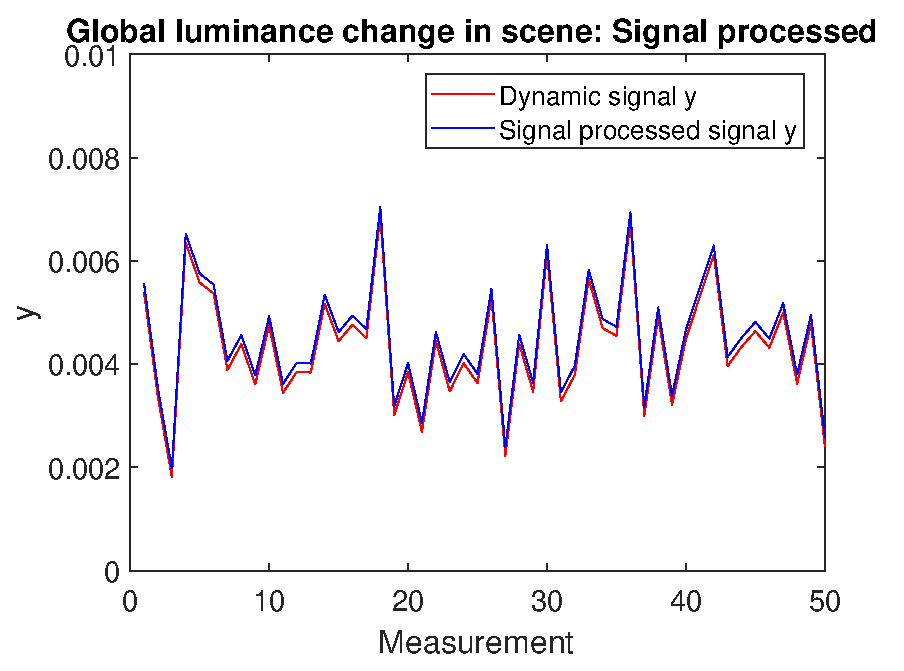
\includegraphics[width = \textwidth]{result/dynamic/lum/intense_change_sp_ref_win.eps}
    \subcaption{Zoomed in view of the signal.}
    \label{fig:lum_sig_4}
\end{minipage}
    \caption{Global movement, acquired signal}
    \label{fig:lum_sig}
\end{figure}

\begin{itemize}
    \item Dynamic signal v. Reference signal
    \item Dynamic signal v. Mean subtracted signal
    \item Reference signal v. Mean subtracted signal
    \item Comment on the window, pretty good.
    \item Can be detected with the knowledge that the signal should be stationary. Signal process the signal to look like a stationary signal.
\end{itemize}

\subsection{SPC evaluation}
\label{sec:eval_spc}

\subsubsection{Soft chessboard}
\todo[inline]{Todo: Skapa rekonstruerade bilder från homagraphin och jämnför de rekonstruerade med referensbilden}
This evaluation is designed to confirm that the images reconstructed by the SPC follows the same characteristics as the reconstruction of the synthetic data.

\begin{figure}[H]
    \centering
    \includegraphics[width=1\linewidth]{result/homo/Hom_im.eps}
    \caption{The reconstructed images with different number of measurements and the reference image transformed to fit the SPC images using homography.}
    \label{fig:hom_over_im}
\end{figure}

\begin{figure}[H]
    \centering
\begin{minipage}[t]{0.49\textwidth}
    \includegraphics[width=1\textwidth]{result/homo/hom_PSNR.eps}
    \subcaption{Peak SNR for reconstructed images against reference image.}
    \label{fig:hom_psnr}
\end{minipage}
\begin{minipage}[t]{0.49\textwidth}
    \includegraphics[width = \textwidth]{result/homo/hom_SNR.eps}
    \subcaption{SNR for reconstructed images against reference image.}
    \label{fig:hom_snr}
\end{minipage}
\begin{minipage}[t]{0.49\textwidth}
    \includegraphics[width=1\textwidth]{result/homo/hom_SSIM.eps}
    \subcaption{SSIM score for reconstructed images against reference image.}
    \label{fig:hom_ssim}
\end{minipage}
    \caption{Signal quality of SPC images compared to reference image}
    \label{fig:hom_score}
\end{figure}


\subsubsection{No reference quality assessment}
Using the no reference quality assessment measurement BRISQUE to evaluate the SPC images. Each image is evaluated at reconstruction rate $5\%$ to $30\%$.

\begin{figure}[H]
    \centering
    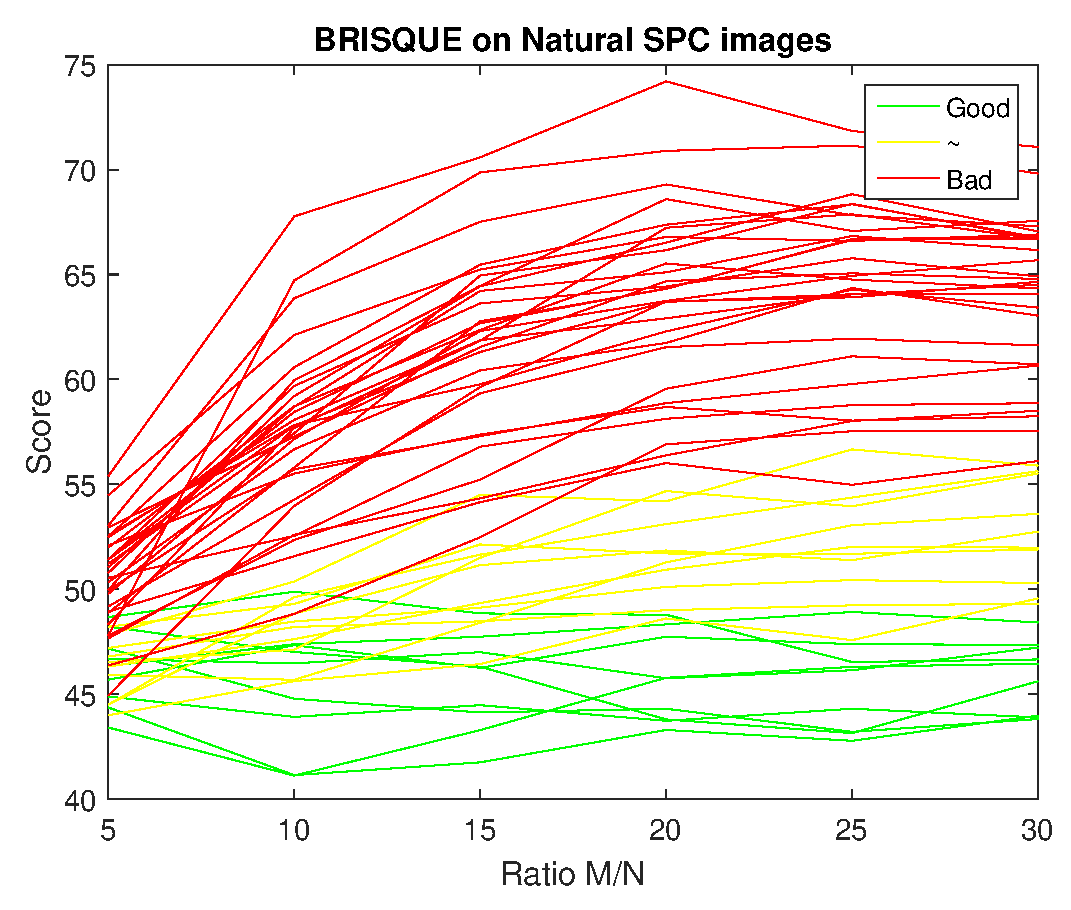
\includegraphics[width = 0.7\linewidth]{result/SPC_NRQA/plot.eps}
    \caption{BRISQUE result.}
    \label{fig:brisque_plot}
\end{figure}

\begin{figure}[H]
    \centering
    \includegraphics[width = 1\linewidth]{result/SPC_NRQA/good.eps}
    \caption{Example of 'good' images corresponding to the green lines in figure~\ref{fig:brisque_plot}.}
    \label{fig:good_plot}
\end{figure}

\begin{figure}[H]
    \centering
    \includegraphics[width = 1\linewidth]{result/SPC_NRQA/half.eps}
    \caption{Example of 'medium good' images corresponding to the yellow lines in figure~\ref{fig:brisque_plot}.}
    \label{fig:half_plot}
\end{figure}

\begin{figure}[H]
    \centering
    \includegraphics[width = 1\linewidth]{result/SPC_NRQA/bad.eps}
    \caption{Example of 'bad' images corresponding to the red lines in figure~\ref{fig:brisque_plot}.}
    \label{fig:bad_plot}
\end{figure}

\begin{itemize}
    \item Good images are:
    \item Medium good images are:
    \item Bad images are:
\end{itemize}


\subsubsection{Modulation Transfer Function}
The MTF is used to comparing the sharpness of cameras and lenses.  

%for two reasons: (1) Image contrast is half its low frequency or peak values,hence detail is still quite visible. The eye is relatively insensitive to detail at spatial frequencies where MTF is low: 10 or less. (2) The response of most cameras falls off rapidly in the vicinity of MTF50 and MTF50P. MTF50P is a better metric for strongly sharpened cameras that have “halos” near edges and corresponding peaks in their MTF response.

The MTF from the SPC is compared to a state of the art SWIR camera. Two scenes was captured by the SPC and a conventional SWIR camera containing printed sheath of paper with simple tilted shapes on them, see figure~\ref{fig:mtf_target}. 



\begin{figure}[H]
    \centering
    \includegraphics[width=0.9\linewidth]{result/mtf/Target.eps}
    \caption{Printed targets with markings where the MTF measurements was performed}
    \label{fig:mtf_target}
\end{figure}

In the resulting images MTF measurements was performed on the specified edges to gather a mean and standard deviation for each camera. For the SPC, images reconstructed from 5\% to 30\% was tested in order to see if the number of measurements effected the MTF result. In figure~\ref{fig:mtf_target_im} the images from the SWIR camera and SPC are presented.

\begin{figure}[H]
    \centering
    \includegraphics[width=1\linewidth]{result/mtf/Target_im.eps}
    \caption{SPC and state of the art SWIR camera output images. (OBS! Bilder från Raptorn ska läggas till)}
    \label{fig:mtf_target_im}
\end{figure}


\subsection{MTF}


\begin{figure}[H]
    \centering
    \begin{minipage}{0.49\textwidth}
    \includegraphics[width=1\textwidth]{result/mtf/mtf30.eps}
    \subcaption{MTF30 result.}
    \label{fig:mtf30}
\end{minipage}
\begin{minipage}{0.49\textwidth}
    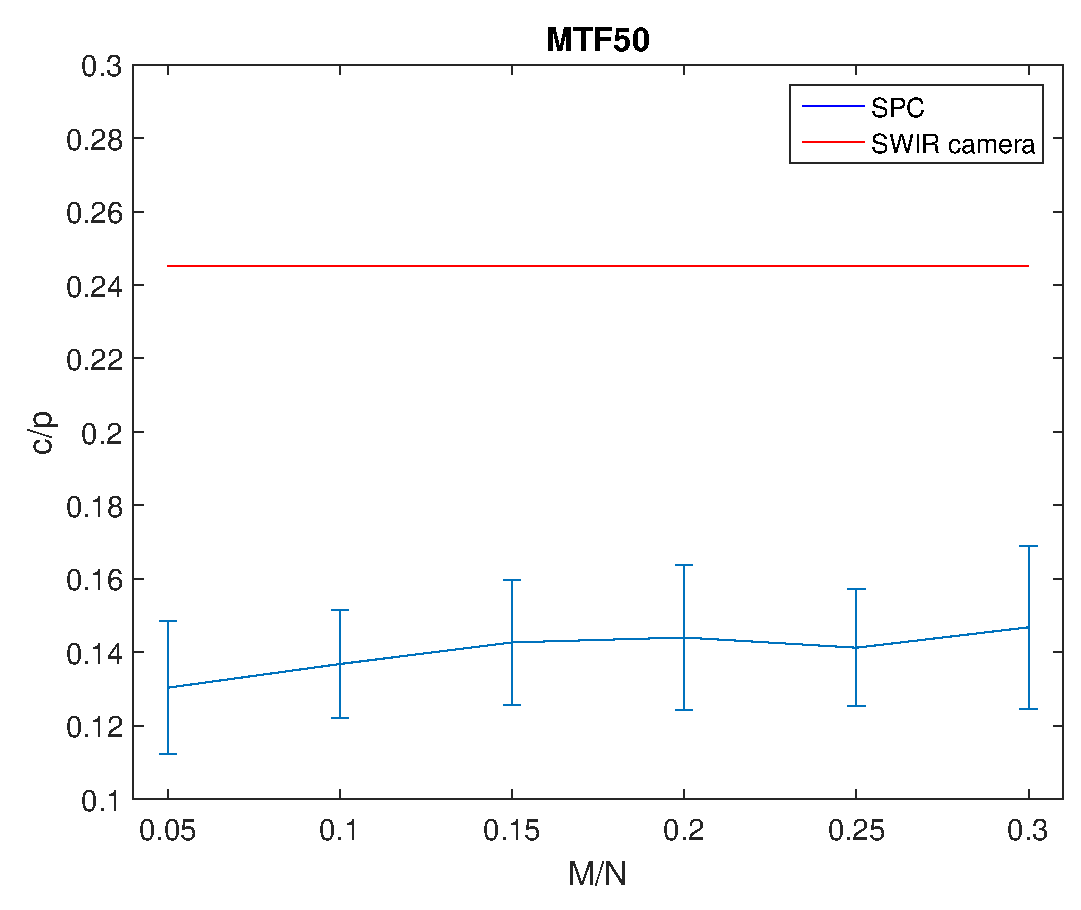
\includegraphics[width = \textwidth]{result/mtf/mtf50.eps}
    \subcaption{MTF50 result.}
    \label{fig:i2}
\end{minipage}
    \caption{MTF results. (OBS! inte rätt figurer)}
    \label{fig:mtf50}
\end{figure}

\subsection{Edge response}
The edge response is measured in the distance (pixels) required for the edge to rise from $10\%$ to $90\%$. In figure~\ref{fig:rise} the result from the experiment in presented. 

\begin{figure}[H]
    \centering
    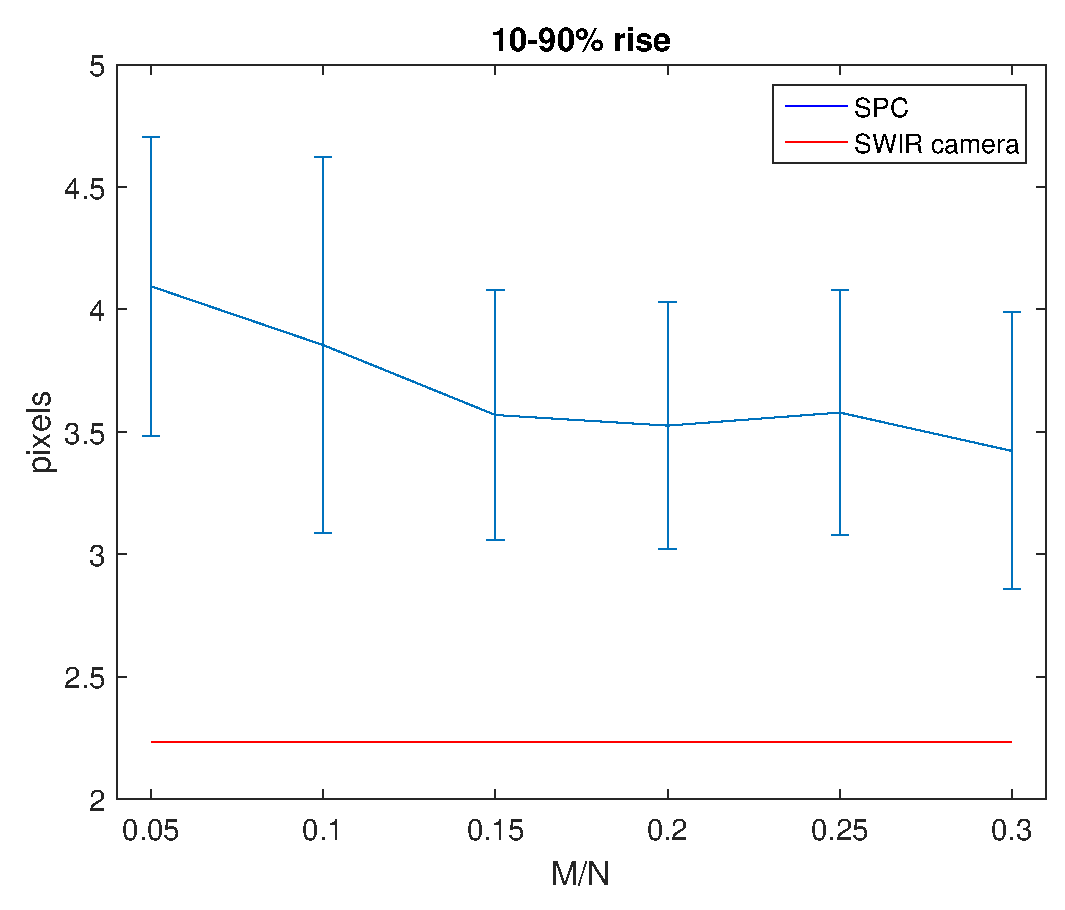
\includegraphics[width=0.5\linewidth]{result/mtf/10-90_rise.eps}
    \caption{10-90\% rise in pixels. (OBS! inte rätt figur)}
    \label{fig:rise}
\end{figure}







\subsubsection{Dynamics in scene}
\label{sec:dyn_sim}
In the SPC setup, the exposure time was between 10 to 50 seconds, which increased the risk of dynamics in the scene. Dynamics in the scene reduces the reconstruction performance because the scene is assumed to be constant. By simulating dynamic scenes in a controlled environment, their individual effects to the sampled signal $\mathbf{y}$ could be identified and evaluated. As mentioned in section~\ref{sec:Dynamics_in_scene} dynamics in the scene can roughly be divided into two separate categories, luminance change and movement. In this section, global luminance change and two kinds of movement are simulated. The goal was to see how the signal changes when dynamics are introduced in the scene. In the case of luminance change, the moving mean algorithm presented in section~\ref{sec:Dynamics_in_scene} was evaluated.\\[0.1in]

To generate a simulated measurement representing a dynamic scene each sample $\mathbf{y}[m]$ is constructed using a unique image $\mathbf{x}_m$, which has been changed from the previous image,

\begin{equation}
\mathbf{y}[m] = \mathbf{\phi}_m\mathbf{x}_m.
\end{equation}

In the first scenario an object was placed in an image, but for each measurement the location of the object was be moved in a small bounded area of the image. Consequently, his model represents a scene where the background is static with a person moving in a small area.



\begin{figure}[H]
    \centering
\advance\leftskip-2cm
\begin{minipage}[t]{0.65\textwidth}
    \includegraphics[width=1\textwidth]{result/dynamic/local/local_whole_time1.eps}
    \subcaption{}
    \label{fig:local_sig_1}
\end{minipage}
\advance\rightskip-2.0cm
\begin{minipage}[t]{0.55\textwidth}
    \includegraphics[width = \textwidth]{result/dynamic/local/local_whole_time_win1.eps}
    \subcaption{}
    \label{fig:local_sig_2}
\end{minipage}
    \caption{(a) Pertubated signal from local movement on top of reference signal. (b) Zoomed in view of some samples from figure (a).}
    \label{fig:local_sig}
\end{figure}

As seen in figure~\ref{fig:local_sig_1} there was no obvious difference between the non perturbed reference signal and the distorted signal. Neither in the zoomed in view in figure~\ref{fig:local_sig_2}, any large difference can be seen.\\[0.1in]

The reconstructed images from the reference signal and the perturbed signal are displayed in figure~\ref{fig:local_2} and \ref{fig:local_3}, respectively. The difference between the images are visible to the naked eye. Not only does the moving object get blurry and noisy, but the whole image globally.


\begin{figure}[H]
    \centering
\begin{minipage}[t]{0.32\textwidth}
    \includegraphics[width=1\textwidth]{result/dynamic/local/local_whole_time_org.png}
    \subcaption{}
    \label{fig:local_1}
\end{minipage}
\begin{minipage}[t]{0.32\textwidth}
    \includegraphics[width = \textwidth]{result/dynamic/local/local_whole_time_ref.png}
    \subcaption{}
    \label{fig:local_2}
\end{minipage}
\begin{minipage}[t]{0.32\textwidth}
    \includegraphics[width = \textwidth]{result/dynamic/local/local_whole_time_res_psnr_29_snr_25_sssim_91.png}
    \subcaption{}
    \label{fig:local_3}
\end{minipage}
    \caption{The results of local movement in a reconstructed image, subsampled at 30\%. (a) Original reference image. (b) Reference image reconstructed from the original image without movement. (c) Reconstructed image from a scene with local movement.}
    \label{fig:local_dyn}
\end{figure}

In table~\ref{tab:local_dyn} the results from calculating PSNR and SSIM of the the reconstructed images are presented. It can be observed that the dynamic test image has been affected to some degree by the movement.

\begin{table}[H]
    \centering
  \begin{tabular}{ | l | l |}
    \hline
    Peak SNR  & SSIM \\ \hline
    29  & 0.91 \\ 
    \hline
  \end{tabular}
      \caption{Evaluation comparing a unperturbed reconstructed images against reconstructed images with local movement.}
    \label{tab:local_dyn}
\end{table}


%The conclusion of this test implies that local movement in a scene will cause noise in the image globally and especially locally where the movement occurred. It also implies that local movement is very hard to detect in the signal even if a reference signal is available.\\[0.1in]



%%%%%%%%%% Second scenario %%%%%%%%%%%%%%%%

The second scenario is an object passing through the whole scene. The problem is modeled with a static background and a simulated object crossing the whole scene, like a car, human or animal might do when using the SPC. The object will cross the scene in 1000 measurements of approximately 19000 in total which corresponds to approximately $0.7$ seconds, when sampling with the SPC in its current setup.\\[0.1in]



\begin{figure}[H]
    \centering
\begin{minipage}[t]{0.53\textwidth}
    \includegraphics[width=1\textwidth]{result/dynamic/fly/flyby_sig1.eps}
    \subcaption{}
    \label{fig:fly_sig_1}
\end{minipage}
\begin{minipage}[t]{0.46\textwidth}
    \includegraphics[width = \textwidth]{result/dynamic/fly/flyby_plot_win1.eps}
    \subcaption{}
    \label{fig:fly_sig_2}
\end{minipage}
    \caption{(a) Pertubated signal from large movement on top of the reference signal. (b) Zoomed in view of some samples from figure (a).}
    \label{fig:fly_sig}
\end{figure}

As seen in figure~\ref{fig:fly_sig}, at measurement 1000 the exact moment the object enters the scene, the signal changes. This is because a completely new structure has entered the scene and therefore the DC level changes. It can also be noted that after a while the object passed something which has approximately the same intensity as the background and therefore the DC signal almost returns to its original value for a brief moment.\\[0.1in] 

In figure~\ref{fig:fly_dyn} the effect of the moving object can be seen in the reconstructed image, which has gained a lot of global noise. Note that the object passing trough can not be seen because there is more measurements of the background than of the moving object. Nevertheless, the object is creating uncertainty in the whole image, resulting in global noise.   

\begin{figure}[H]
    \centering
\begin{minipage}[t]{0.32\textwidth}
    \includegraphics[width=1\textwidth]{result/dynamic/fly/flyby_1sec_org.png}
    \subcaption{}
    \label{fig:fly_1}
\end{minipage}
\begin{minipage}[t]{0.32\textwidth}
    \includegraphics[width = \textwidth]{result/dynamic/fly/flyby_1sec_ref.png}
    \subcaption{}
    \label{fig:fly_2}
\end{minipage}
\begin{minipage}[t]{0.32\textwidth}
    \includegraphics[width = \textwidth]{result/dynamic/fly/flyby_1sec_res_psnr_23_snr_18_sssim_58.png}
    \subcaption{}
    \label{fig:fly_3}
\end{minipage}
    \caption{The results of large movement on a reconstructed image, subsampled at 30\%. (a) Original reference image. (b) Reference image reconstructed from the original image without movement. (c) Reconstructed image from a scene with an object passing trough.}
    \label{fig:fly_dyn}
\end{figure}

In table~\ref{tab:fly_dyn} the results from calculating PSNR and SSIM of the reconstructed images are presented. It can be observed that the image has been effected heavily by the movement, lowering the SSIM index to 0.58. 


\begin{table}[H]
    \centering
  \begin{tabular}{ | l | l |}
    \hline
    Peak SNR  & SSIM \\ \hline
    23 &  0.58 \\ 
    \hline
  \end{tabular}
      \caption{Evaluation comparing unperturbed reconstructed image against reconstructed image with movement.}
    \label{tab:fly_dyn}
\end{table}


%Obviously in this context the samples with movement is very easy to spot and the easiest fix would be to just remove those measurements, reconstructing an image with fewer measurements. The resulting image would not be as good as the image in figure~\ref{fig:fly_2} but it would not be contain the noise present in figure~\ref{fig:fly_3}.\\[0.1in]



%%%%%%%%%%%% Third %%%%%%%%%%%%%%%

The third scenario is luminance change in the scene caused by inconsistency of light intensity from the source. Outdoors this means that the light intensity from the sun will vary over time, the most obvious being clouds occluding the sun but for example even change in air density can change the intensity. This scenario is modeled by adding or subtracting the global intensity in the image over the measurements. 

\begin{figure}[H]
    \includegraphics[width=0.6\textwidth]{result/dynamic/lum/intense_change1.eps}
    \caption{Signal effected by light intensity change on top of reference signal.}
    \label{fig:lum_sig_1}
\end{figure}

As seen in figure~\ref{fig:lum_sig_1}, the DC level of the signal will slowly change, but the structure of the signal stay the same. In figure~\ref{fig:lum_dyn} the reconstructed images from the perturbed signal and the reference signal are displayed. The reconstructed image from the dynamic signal has gained a lot of global noise even though the structure in the image has not been changed over the measurements.  


\begin{figure}[H]
    \centering
\begin{minipage}[t]{0.32\textwidth}
    \includegraphics[width=1\textwidth]{result/dynamic/lum/intense_change_org.png}
    \subcaption{}
    \label{fig:lum_1}
\end{minipage}
\begin{minipage}[t]{0.32\textwidth}
    \includegraphics[width = \textwidth]{result/dynamic/lum/intense_change.png}
    \subcaption{}
    \label{fig:lum_2}
\end{minipage}
\begin{minipage}[t]{0.32\textwidth}
    \includegraphics[width = \textwidth]{result/dynamic/lum/intense_change_psnr_19_snr_14_sssim_38.png}
    \subcaption{}
    \label{fig:lum_3}
\end{minipage}
    \caption{The result of global light intensity change on a reconstructed image subsampled at 30\% (a) Original reference image. (b) Reference image reconstructed from the original image without light intensity change. (c) Reconstructed image from a scene with global light intensity change over the measurements.}
    \label{fig:lum_dyn}
\end{figure}

In section~\ref{sec:Dynamics_in_scene}, a model of this problem was proposed along with an algorithm to suppress the impact of global luminance change. The algorithm is applied to this experiment to evaluate its performance. The moving mean subtraction method is applied and in figure~\ref{fig:lum_sig_2} the resulting signal is plotted over the dynamic signal. Note that the processed signal is stationary again. In figure~\ref{fig:lum_sig_3} and \ref{fig:lum_sig_4}, where the processed signal is plotted over the reference signal, it can be seen that the processed signal has gained its original structure and almost fit exactly to the original.


\begin{figure}[H]
    \centering
\begin{minipage}[t]{0.48\textwidth}
    \includegraphics[width = \textwidth]{result/dynamic/lum/intense_change_sp.eps}
    \subcaption{}
    \label{fig:lum_sig_2}
\end{minipage}
\begin{minipage}[t]{0.51\textwidth}
    \includegraphics[width=1\textwidth]{result/dynamic/lum/intense_change_sp_ref1.eps}
    \subcaption{}
    \label{fig:lum_sig_3}
\end{minipage}
\begin{minipage}[t]{0.50\textwidth}
    \includegraphics[width = \textwidth]{result/dynamic/lum/intense_change_sp_ref_win.eps}
    \subcaption{}
    \label{fig:lum_sig_4}
\end{minipage}
    \caption{Post-processed signal using moving mean subtraction. (a) Post-processed signal on top of the dynamic signal. (b) Post-processed signal on top of the reference signal. (c) Zoomed in view of (b).}
    \label{fig:lum_sig}
\end{figure}

In figure~\ref{fig:lum_rec}, the processed signals reconstructed image is displayed between the reference and perturbed signals reconstructed images. The moving mean algorithm improve the reconstruction significantly, the image has gained some noise compared to the reference image, but over all there is not much difference between them.


\begin{figure}[H]
    \centering
\begin{minipage}[t]{0.32\textwidth}
    \includegraphics[width = \textwidth]{result/dynamic/lum/intense_change.png}
    \subcaption{}
    \label{fig:lum_22}
\end{minipage}
\begin{minipage}[t]{0.32\textwidth}
    \includegraphics[width = \textwidth]{result/dynamic/lum/intense_change_movemean_psnr_33_snr_29_sssim_93.png}
    \subcaption{}
    \label{fig:lum_4}
\end{minipage}
\begin{minipage}[t]{0.32\textwidth}
    \includegraphics[width = \textwidth]{result/dynamic/lum/intense_change_psnr_19_snr_14_sssim_38.png}
    \subcaption{}
    \label{fig:lum_32}
\end{minipage}
    \caption{The result of processed signal perturbed by light intensity change on a reconstructed image subsampled at 30\% (a) Reference image reconstructed from the non perturbed signal without light intensity change. (b) Reconstructed image from a scene with global light intensity change and post processed by moving mean subtraction. (c) Reconstructed image from a scene with global light intensity change over the measurements.}
    \label{fig:lum_rec}
\end{figure}

In table~\ref{tab:lum_dyn} the results from calculating PSNR and SSIM of the reconstructed images are presented. Both PSNR and SSIM are increased for the reconstructed image using moving mean subtraction.


\begin{table}[H]
    \centering
  \begin{tabular}{ | l | l | l |}
    \hline
    Signal & Peak SNR  & SSIM \\ \hline
    Perturbed signal & 19  & 0.38 \\ \hline
    Mean subtracted signal & 33  & 0.93 \\
    \hline
  \end{tabular}
      \caption{Evaluation comparing unperturbed reconstructed image against global luminance change reconstructed image and moving mean subtracted signal processed reconstructed image.}
    \label{tab:lum_dyn}
\end{table}







\subsection{SPC evaluation}
\label{sec:eval_spc}

\subsubsection{Number of measurements}
\begin{figure}[H]
\begin{minipage}[t]{0.3\linewidth} %Car
	\includegraphics[width = 1\linewidth]{gfx/car/car_org.png}
	\label{fig:car_org}
\end{minipage}
\begin{minipage}[t]{0.3\linewidth} % Hus
	\includegraphics[width = 1\linewidth]{gfx/hus/hus_org.png}
	\label{fig:hus_org}
\end{minipage}
\begin{minipage}[t]{0.3\linewidth} %Sit
	\includegraphics[width = 1\linewidth]{gfx/sit/sit_org.png}
	\label{fig:sit_org}
\end{minipage}
\end{figure}
\begin{figure}[H]
\vspace*{-1.2cm}
\begin{minipage}[t]{0.3\linewidth} %Car
	\includegraphics[width = 1\linewidth]{gfx/car/car_m5.png}
	\label{fig:car_m5}
\end{minipage}
\begin{minipage}[t]{0.3\linewidth} % Hus
	\includegraphics[width = 1\linewidth]{gfx/hus/hus_m5.png}
	\label{fig:hus_m5}
\end{minipage}
\begin{minipage}[t]{0.3\linewidth} %Sit
	\includegraphics[width = 1\linewidth]{gfx/sit/sit_m10.png}
	\label{fig:sit_m5}
\end{minipage}
\end{figure}
\begin{figure}[H]
\vspace*{-1.2cm}
\begin{minipage}[t]{0.3\linewidth} %Car
	\includegraphics[width = 1\linewidth]{gfx/car/car_m10.png}
	%\subcaption{m15}
	\label{fig:car_m10}
\end{minipage}
\begin{minipage}[t]{0.3\linewidth} % Hus
	\includegraphics[width = 1\linewidth]{gfx/hus/hus_m10.png}
	%\subcaption{m10}
	\label{fig:hus_m10}
\end{minipage}
\begin{minipage}[t]{0.3\linewidth} %Sit
	\includegraphics[width = 1\linewidth]{gfx/sit/sit_m10.png}
	%\subcaption{m10}
	\label{fig:sit_m10}
\end{minipage}
\end{figure}
\begin{figure}[H]
\vspace*{-1.2cm}
\begin{minipage}[t]{0.3\linewidth} %Car
	\includegraphics[width = 1\linewidth]{gfx/car/car_m15.png}
	\subcaption{m15}
	\label{fig:car_m15}
\end{minipage}
\begin{minipage}[t]{0.3\linewidth} % Hus
	\includegraphics[width = 1\linewidth]{gfx/hus/hus_m15.png}
	\subcaption{m10}
	\label{fig:hus_m15}
\end{minipage}
\begin{minipage}[t]{0.3\linewidth} %Sit
	\includegraphics[width = 1\linewidth]{gfx/sit/sit_m15.png}
	\subcaption{m10}
	\label{fig:sit_m15}
\end{minipage}
\end{figure}
\begin{figure}[H]
\vspace*{-1.2cm}
\begin{minipage}[t]{0.3\linewidth} %Car
	\includegraphics[width = 1\linewidth]{gfx/car/car_m20.png}
	%\subcaption{m15}
	\label{fig:car_m20}
\end{minipage}
\begin{minipage}[t]{0.3\linewidth} % Hus
	\includegraphics[width = 1\linewidth]{gfx/hus/hus_m20.png}
	%\subcaption{m10}
	\label{fig:hus_m20}
\end{minipage}
\begin{minipage}[t]{0.3\linewidth} %Sit
	\includegraphics[width = 1\linewidth]{gfx/sit/sit_m20.png}
	%\subcaption{m10}
	\label{fig:sit_m20}
\end{minipage}
\end{figure}
\begin{figure}[H]
\begin{minipage}[t]{0.3\linewidth} %Car
	\includegraphics[width = 1\linewidth]{gfx/car/car_m25.png}
	%\subcaption{m15}
	\label{fig:car_m25}
\end{minipage}
\begin{minipage}[t]{0.3\linewidth} % Hus
	\includegraphics[width = 1\linewidth]{gfx/hus/hus_m25.png}
	%\subcaption{m10}
	\label{fig:hus_m25}
\end{minipage}
\begin{minipage}[t]{0.3\linewidth} %Sit
	\includegraphics[width = 1\linewidth]{gfx/sit/sit_m25.png}
	%\subcaption{m20}
	\label{fig:sit_m25}
\end{minipage}
\end{figure}
\begin{figure}[H]
\vspace*{-1.2cm}
\begin{minipage}[t]{0.3\linewidth} %Car
	\includegraphics[width = 1\linewidth]{gfx/car/car_m30.png}
	%\subcaption{m15}
	\label{fig:car_m30}
\end{minipage}
\begin{minipage}[t]{0.3\linewidth} % Hus
	\includegraphics[width = 1\linewidth]{gfx/hus/hus_m30.png}
	%\subcaption{m10}
	\label{fig:hus_m30}
\end{minipage}
\begin{minipage}[t]{0.3\linewidth} %Sit
	\includegraphics[width = 1\linewidth]{gfx/sit/sit_m30.png}
	%\subcaption{m10}
	\label{fig:sit_m30}
\end{minipage}
	\caption{Images reconstructed using $M/N = 5\% \text{ to } 30\%$ measurements from top down.} 
\end{figure}

\subsubsection{Soft chessboard}
\todo[inline]{Todo: Skapa rekonstruerade bilder från homagraphin och jämnför de rekonstruerade med referensbilden}
This evaluation is designed to confirm that the images reconstructed by the SPC follows the same characteristics as the reconstruction of the synthetic data.


\begin{figure}[H]
    \centering
\begin{minipage}[h]{0.3\textwidth}
	\vspace*{1cm}
    \includegraphics[width=1\textwidth]{result/hom/im_ref.png}
    \subcaption{Refrence image}
    \label{fig:hom_ref}
\end{minipage}
\begin{minipage}[t]{0.22\textwidth}
    \includegraphics[width = \textwidth]{result/hom/im_m5.png}
    \subcaption{5\%}
    \label{fig:hom_5}
    \includegraphics[width = \textwidth]{result/hom/im_m20.png}
    \subcaption{20\%}
    \label{fig:hom_20}
\end{minipage}
\begin{minipage}[t]{0.22\textwidth}
    \includegraphics[width = \textwidth]{result/hom/im_m10.png}
    \subcaption{10\%}
    \label{fig:hom_10}
    \includegraphics[width = \textwidth]{result/hom/im_m25.png}
    \subcaption{25\%}
    \label{fig:hom_25}
\end{minipage}
\begin{minipage}[t]{0.22\textwidth}
    \includegraphics[width = \textwidth]{result/hom/im_m15.png}
    \subcaption{15\%}
    \label{fig:hom_15}
    \includegraphics[width = \textwidth]{result/hom/im_m30.png}
    \subcaption{30\%}
    \label{fig:hom_30}
\end{minipage}

    \caption{The reconstructed images with different number of measurements and the reference image transformed to fit the SPC images using homography.}
    \label{fig:hom_over_im}
\end{figure}


\begin{figure}[H]
    \centering
\begin{minipage}[t]{0.49\textwidth}
    \includegraphics[width=1\textwidth]{result/homo/PSNR_2.eps}
    \subcaption{}
    \label{fig:hom_psnr}
\end{minipage}
\begin{minipage}[t]{0.49\textwidth}
    \includegraphics[width=1\textwidth]{result/homo/SSIM_2.eps}
    \subcaption{}
    \label{fig:hom_ssim}
\end{minipage}
    \caption{Signal quality of SPC images compared to reference image. (a) Peak SNR for reconstructed images against reference image. (b) SSIM score for reconstructed images against reference image.}
    \label{fig:hom_score}
\end{figure}


\subsubsection{No reference quality assessment}
Using the no reference quality assessment measurement BRISQUE to evaluate the SPC images. Each image is evaluated at reconstruction rate $5\%$ to $30\%$.

\begin{figure}[H]
    \centering
    \includegraphics[width = 0.7\linewidth]{result/SPC_NRQA/brisque_spc.eps}
    \caption{BRISQUE result.}
    \label{fig:brisque_plot}
\end{figure}

\begin{figure}[H]
    \centering
    \includegraphics[width = 1\linewidth]{result/SPC_NRQA/good.eps}
    \caption{Example of 'good' images corresponding to the green lines in figure~\ref{fig:brisque_plot}.}
    \label{fig:good_plot}
\end{figure}

\begin{figure}[H]
    \centering
    \includegraphics[width = 1\linewidth]{result/SPC_NRQA/half.eps}
    \caption{Example of 'medium good' images corresponding to the yellow lines in figure~\ref{fig:brisque_plot}.}
    \label{fig:half_plot}
\end{figure}

\begin{figure}[H]
    \centering
    \includegraphics[width = 1\linewidth]{result/SPC_NRQA/bad.eps}
    \caption{Example of 'bad' images corresponding to the red lines in figure~\ref{fig:brisque_plot}.}
    \label{fig:bad_plot}
\end{figure}

\begin{itemize}
    \item Good images are: Strong light, No movement in the image
    \item Medium good images are: Good light, Movement, Brisque bad?
    \item Bad images are: Can have bad light, movement 
\end{itemize}


\subsubsection{Modulation Transfer Function}
The MTF is used to comparing the sharpness of cameras and lenses.  

%for two reasons: (1) Image contrast is half its low frequency or peak values,hence detail is still quite visible. The eye is relatively insensitive to detail at spatial frequencies where MTF is low: 10 or less. (2) The response of most cameras falls off rapidly in the vicinity of MTF50 and MTF50P. MTF50P is a better metric for strongly sharpened cameras that have “halos” near edges and corresponding peaks in their MTF response.

The MTF from the SPC is compared to a state of the art SWIR camera. Two scenes was captured by the SPC and a conventional SWIR camera containing printed sheath of paper with simple tilted shapes on them, see figure~\ref{fig:mtf_target}. 



\begin{figure}[H]
    \centering
    \includegraphics[width=0.9\linewidth]{result/mtf/Target.eps}
    \caption{Printed targets with markings where the MTF measurements was performed}
    \label{fig:mtf_target}
\end{figure}

\begin{figure}[H]
    \centering
\begin{minipage}[t]{0.45\textwidth}
    \includegraphics[width=1\textwidth]{result/mtf/swir2.png}
    \subcaption{}
    \label{fig:mtf_s2}
\end{minipage}
\begin{minipage}[t]{0.45\textwidth}
    \includegraphics[width=1\textwidth]{result/mtf/spc22.png}
    \subcaption{}
    \label{fig:mtf_spc2}
\end{minipage}
\begin{minipage}[t]{0.45\textwidth}
    \includegraphics[width=1\textwidth]{result/mtf/swir1.png}
    \subcaption{}
    \label{fig:mtf_s1}
\end{minipage}
\begin{minipage}[t]{0.45\textwidth}
    \includegraphics[width=1\textwidth]{result/mtf/spc12.png}
    \subcaption{}
    \label{fig:mtf_spc1}
\end{minipage}
    \caption{SPC and state of the art SWIR camera output images.}
    \label{fig:mtf_target_im}
\end{figure}

In the resulting images MTF measurements was performed on the specified edges to gather a mean and standard deviation for each camera. For the SPC, images reconstructed from 5\% to 30\% was tested in order to see if the number of measurements effected the MTF result. In figure~\ref{fig:mtf_target_im} the images from the SWIR camera and SPC are presented.



\todo[inline]{Light source 135W from 2m. Image on the board}


The edge response is measured in the distance (pixels) required for the edge to rise from $10\%$ to $90\%$. In figure~\ref{fig:rise} the result from the experiment in presented. 

\begin{figure}[H]
    \centering
    \includegraphics[width=0.7\linewidth]{result/mtf/Rise10_90.eps}
    \caption{10-90\% rise in pixels.}
    \label{fig:rise}
\end{figure}

\subsection{Noise analysis}

\section{Discussion} %Resultat ska inte analyseras, diskuteras eller värderas. Detta lämnas till diskussionskapitlet. 
\label{sec:discussion}
In this section the results and method is analyzed and discussed. When discussing results a focus on consistency, relation to theory and real world applicability is held. In the discussion of method an analysis of replicability, reliability and  validity is held.

\subsection{Result} 
%Finns det något i resultaten som står ut och behöver analyseras och kommenteras? Hur förhåller sig resultaten till det material som togs upp i teorigenomgången? Vad säger teorin om vad resultaten egentligen betyder? Vad innebär det till exempel att man vid en användbarhetsmätning av ett nytt system fått ett visst värde; hur bra eller dåligt är det? Finns det något i resultaten som är oväntat baserat på teorigenomgången, eller stämmer det bra överens med vad man teoretiskt kunde förvänta sig? 
Overall the results obtained in this thesis reflects what has been stated in the theory and research, but no reference to the use of SPC in natural environment could be found and thus this thesis will present the link between real world application and theory/lab results and the challenges that come with it. 



\subsubsection{Reconstruction performance Using reference image}
\label{sec:anlys_ref_im}
%Sec:reconstruction performance using ref im
%A second observation is that, when the noise increases the  reconstructed image quality is not improved at the same rate as the noiseless case when increasing the sub sampling ratio.
In the simulated reconstruction the results behaved in most part as expected given the CS theory, with increased subsampling ratio the performance increased. But the interesting part of this results is whats happening when increasing the noise, not only does the general performance drop for all subsample ratios, but also the improvement rate by increasing the subsample ratio drops, which figure~\ref{fig:snr} and \ref{fig:ssim_3d} shows. This result tells us that if the signal contains a high degree of noise, a larger subsampling ratio may not improve the reconstructed image as mush as expected.\\[0.1in]

When obtaining the same measurements with the SPC one low frequency image was captured and reconstructed, with near optimal SNR and environment such that a homography between the reconstructed image and reference image could be made with good precision. In figure~\ref{fig:hom_psnr} and \ref{fig:hom_ssim} we can see the PSNR and SSIM of the image given the reference image, as expected from theory and confirmed in the simulated case the performance increases when the subsampling ratio increases. But if we look closer at the PSNR plot we can see that the largest increase in performance is up to 15\% subsampling ratio, which can be confirmed when inspecting the images in figure~\ref{fig:hom_5}-\ref{fig:hom_30}, where the image quality rapidly improves when increasing subsample ratio up to 15\%, then the improvement rate stagnates.


\subsubsection{Reconstruction performance Using no reference quality assessment}
For the simulated reconstruction in figure~\ref{fig:Brisque_3d}, we can see that the graph looks like a upside down version of the PSNR and SSIM graphs of the simulated images. This results alone is positive for this theses because it was unknown if this method would work well for SWIR images and reconstructed images. An observation that can be made, is that the reference images score about 20 BRISQUE points better then the best reconstructed images and we can conclude that the sampling and reconstruction even in the best case scenario without noise, will not be as good as an conventional camera. We can see from the plot that in the ideal case the score will not be better then approximately 40 BRISQUE points for the reconstructed images while the SWIR images has a mean value of 15. We can concluded from this result that, with the current measurement matrix and reconstruction method, around 40 in BRISQUE score is what to expect as optimum given that the SPC will induce some noise to the signal.\\[0.1in]
%When studying the more sparse 2D plot in figure~\ref{fig:Brisque_2d}, the observations from section~\ref{sec:anlys_ref_im} is confirmed that the improvement in image quality  


When studying the plot with BRISQUE score given by the results from images reconstructed from the SPC in figure~\ref{fig:brisque_plot}, we can see that the best images score just over 40 BRISQUE points, which is the same score as score as simulated images with small or no nois added, which means that the SPC can compare to the benchmark set by the simulation and thus gives a theoretical optimal reconstuction given the measurement matrix and reconstruction algorithm. Furthermore we can see that the trend of the images follows the same characteristics as the simulation in figure~\ref{fig:Brisque_2d} for different noise levels, thus we can conclude that simulations gives a good indication of where the real images will score given a noise level.\\[0.1in]

In figure~\ref{fig:good} to \ref{fig:bad}, we see the images divided into three classes given their BRISQUE score and trend as described in section~\ref{sec:SPC_BRISQUE}. As the BRISQUE score tells, the quality of the images should vary a lot, and when taking a closer look the "bad" data set in figure~\ref{fig:bad} stands out the most. My analysis of why the BRISQUE score and image quality differ is, 

\begin{itemize}
\item first if we take a look at the images in figure~\ref{fig:good} and \ref{fig:half}, where the image quality and lighting look quiet the same but yet differ so much in the BRISQUE score, it might be a property of the BRISQUE classifer. The BRISQUE classifier is built to assess image quality in natural images, and if we take a look at the main difference between these two data sets we can see that one is pictures of a car, humans, forest and clothing and the other mainly of buildings and large structure in the images with little change i.e. not so natural, which can effect the score.

\item The major difference between figure~\ref{fig:good} - \ref{fig:half} and \ref{fig:bad} is that the latter appears to contain a lot more global noise. The increase in global noise arises from two separate sources, the fist one being luminance in the scene, we can see that the images in figure~\ref{fig:half1} and \ref{fig:bad1} is practically the same motive, but the latter is darker. The darker scene was shot in morning when the sun was not so bright and did not luminate the facade directly and thus the signal was weaker and the resulting reconstruction was effected more by the sensors background noise and gave rise to global noise in the produced image. 

\item The second reason is large structure movement in the scene, most of the images in the "bad" image set had movement mainly from clouds when sampled which definitely increased global noise in the reconstructed images as concluded in section~\ref{sec:Dynamics_in_scene} and therefore decreased the BRISQUE score significantly.

\end{itemize}

In the last part of section~\ref{sec:SPC_BRISQUE} the results from plotting SNR and standard deviation against mean signal intensity in figure~\ref{fig:snr}, was presented. Each data point had also been color coded to match the classification made previously, the plots gave more information on why the BRISQUE score was so deviated. From the plot in figure~\ref{fig:snr_v_sigma} it becomes very clear at which mean signal intensity we can expect to produce good images given that the background noise becomes insignificant. But in the plots there are only two signals with higher variance than 0.04, which is the threshold where the the simulated images started to get both worse initial BRISQUE score and worse trend when increasing the subsampling ratio in figure~\ref{fig:Brisque_2d}. This implies that there probably must be at least one additional factor at play to reduce the image quality in the "bad" set.\\[0.1in]


We can see that there are a subset of red images with almost the same SNR and mean signal intensity as yellow and green images but yields a worse BRISQUE score anyway, this strengthening the statement the there is probably at least on more factor that reduces reconstruction performance. And as stated in the last paragraph this is probably due to motion in the scene when sampling the signal. Unfortunately for this experiment, it seams like the images containing motion also had a low mean signal intensity, otherwise we would probably also have "bad" images for stronger mean signals.\\[0.1in] 

The last observation in these plots are the mix of "good" and "half good" images in the whole mean intensity span, which tells that a strong signal will not yield a good BRISUQE score, which implies that the motive in the images effecting the BRISQUE score as suspected in when inspecting the reconstructed image sets.

\subsubsection{Dynamics in scene}
In this category there are results both from the simulated images and from the SPC, where the results was divided into three characteristic dynamics: small local changes in the scene, large global changes and luminance change.\\[0.1in]

The effect on the signal of local movements result shown in figure~\ref{fig:local_dyn}, we can see that there is no significant difference between the non perturbed reference signal and the distorted signal. It can even be interpreted as added noise to the signal and it is barely detectable even if the signal is known. The effect on the reconstructed image, seen in figure~\ref{fig:local_1}, looks like global noise is added. The conclusion of that test implies that local movement in a scene will distort the reconstructed image globally and especially locally where the movement occurred. It also tells that local movement is very hard to detect in the signal even if a reference signal is available.\\[0.1in]

When increasing the movement and modeled an unseen object pass through, the samples with movement was very easy to spot, which figure~\ref{fig:local_sig_2} shows. The effect in the reconstructed image is as expected even worse then local movement, with a global distortion, seen in figure~\ref{fig:local_2}. In this simple isolated case the image could be saved by removing the measurements when the object was moving, reconstructing an image with fewer measurements. The resulting image would not be as good as the image in figure~\ref{fig:fly_2} but it would not contain the noise present in figure~\ref{fig:fly_3}. \\[0.1in]


%Comment luminance change case ?
In the case of luminance change, the effect on the reconstructed image is even worse than scenes containing movement, which figure~\ref{fig:local_3} and comparing table~\ref{tab:local_dyn}, \ref{tab:fly_dyn} and \ref{tab:lum_dyn}. Because we know that this problem is real and can not be avoided in natural scenes, a model to suppress this issue was tested with good result, but as can be seen in figure~\ref{fig:lum_sig_3}, \ref{fig:lum_dyn} and table~\ref{tab:lum_dyn}, the method will not suppress the effect completely even on a simulation and thus add some global noise in the same form as local movement will.\\[0.1in]

% SPC
When capturing images using the SPC, the luminance change became a larger problem than anticipated. All image captured in natural lighting had luminance change and it changed at a higher frequency and larger amplitude even in scenes where the intensity seemed stationary. This is of course due to the fact that the intensity change from every mirror in the DMD is summed in the sensor, so even for small changes the sum will change the signal significantly, as seen in figure~\ref{fig:lc_plot}. But as seen in the results in figure~\ref{fig:lc_image}, the moving average method worked despite the more complex changes to the signal. Considering that this problem was consistent for all natural images this method became essential for this thesis to produce any good result at all. As stated before, this method is an model of global luminance change in the image, and therefore it is hard to know which side effects this method have on image quality. But as the test show, the method is essential and was used for all images captured by the SPC and presented and evaluated in this thesis.\\[0.1in]

This method was mainly constructed because I knew the SPC would have a long exposure time, but even if the exposure time is reduced to a a few seconds or less, there is some indication that the luminance change will still effect the result. In this thesis, the moving average window corresponded to 50 milliseconds which indicates that the luminance change is so fast that even reducing exposure time could benefit to this method.\\[0.1in]


Basically all scenes i natural environment contained both dynamics from local movement and luminance change, local movement often arose from vegetation, objects or clouds moving in the wind but also from turbulence which not move the object but how it is perceived on the DMD. Because of all the dynamics presented that is persistent even in a "static" scene, I decided to not photograph scenes where large movement occurred as a car, object or human, even though it could be detected, because it could also be detected as luminance change.\\[0.1in]

As stated, even "static" scenes will with high probability contain both movement and luminance change which will effect the reconstructed images. Therefor I can conclude that all reconstructed images in this thesis has to some degree added global noise from local movement and the signal processing to counter luminnnce change.


\subsubsection{Edge response}
When comparing the edge response between the conventional camera against the SPC the results was very clear, the conventional camera outperformed the SPC with one to two pixels in distance. I think there are multiple factors why the results from the SPC differed so much from the conventional camera, and have listed them below,

\begin{itemize}
\item The largest impact on image quality is probably the reconstruction algorithm which produces "patches", which can be seen in the SPC images in figure~\ref{fig:mtf_target_im}, especially in the contrast of the white background where the light intensity drops. The "patch" artifact from the reconstruction algorithm can effect the sharpness of the image. We can also see from previous test that even from synthetic data the BRISQUE score is significantly worse then the original image.

\item The pixel grid setup in the DMD has two problems that could effect the sharpness. In the DMD the mirrors is aligned in a diamond shape of pattern and in the current setup to fix the ratio and index two mirrors is merged to form one pixel. The reconstruction algorithm will still interpret the measurement as a regular square pixel which can distort the image.

\item The focus in the DMD is set manually.

\item In this thesis no significant image improvement from post processing such as denoise or sharpening was performed unlike the conventional camera.

\item And as stated before, with the long exposure, vibrations and light intensity change effected the results (the SPC could detect significant light intensity change from the halogen lamp powered by a DC-unit), which contribute to global noise in the reconstruction.

\end{itemize}



\subsubsection{Subsampling ratio}
The first results from section~\ref{sec:measurements} was the minimum subsampling ratio required to reconstruct a merely recognizable image, for the whole image set the results varied between 2-4\%. The variance could be effected by several factors such as image complexity, SNR and dynamics in the scene, which contribute to add uncertainty to the equation system. With the knowledge of minimum subsampling ratio a fast exposure and thus a fast reconstruction could be applied to form a test image, which could be used to calibrate and make decision how to sample the long exposure real image.\\[0.1in]

In the second part of section~\ref{sec:measurements}, a set of images reconstructed with different subsampling ratio was presented. The result is presented for the reader to obtain a more concrete perception of the generated image quality and a supplement to the numerical results given subsampling ratio, but also overall expected image quality.

\subsection{Method} %Vad jag tycker om det (personliga tankar)
%In the discussion of method an analysis of replicability, reliability and  validity is held.

The methods used in thesis can be divided into four categories, the SPC hardware, the sampling matrix and reconstruction, post processing and the method used to capture the images. Two of these categories, the hardware setup and the sampling matrix and reconstruction was heavily influenced and implemented by widely accepted methods from articles and experiments. While the two other categories, the post process and the image capturing dependent more on the hardware limitation and competence achieved from the university.\\[0.1in]

The first method in the chain was feeding the DMD measurement matrices and sampling the signal. Because of the interface to the DMD, which acted as a second monitor to the computer, the method to stream the measurement matrices as a video was thought to be a good method because it was easy to implement. In the early stages of this thesis a much smaller resolution of $128 \times 128$ pixels was thought to be a feasible maximum and thus much less measurement matrices needed to be streamed to the DMD while having the same exposure time. With that initial goal in mind the video player steaming method would have worked well. But when the target resolution was pushed the video players frame rate had to be pushed to its limits in an application it was not designed to handle. This resulted in a higher probability that the video player would go out of sync and thus ruin the reconstruction and there was no way of knowing if this had happen. By the time this issue was discovered there where no time of changing and implement a new method but was much needed.\\[0.1in]

The sampling matrix chosen in this thesis was the sequency ordered Walsh Hadamard measurement matrix, this sampling matrix in unison with implemented fast transform in the reconstruction algorithm enabled the huge increase in image resolution. This method of using structurally random matrices is the only feasible method today to enable high resolution and fast reconstruction with low memory usage in the computer thus if implemented optimally both the feeding of measurement matrices to the DMD and reconstruction could be calculated in run time in a memory efficient program.\\[0.1in]

The reconstruction algorithm TVAL3 was used throughout this masters thesis and was chosen after the literature study where several articles mentioned total variation as a good optimization algorithm for compressive imaging. The algorithm worked as described and according to the developer and is one of the fastest and best reconstruction algorithms that are free to use and available. The only negative criticism of using this algorithm is that it seems to produce a dark tint in the edges of the reconstructed images.\\[0.1in]

In the post process quite basic signal and image processing was performed and was intentional designed that way in order to present the result as true as possible. One algorithm was developed specific for the SPC which was the average mean algorithm to suppress the impact of lumination change in the sampled signal. The algorithm showed great result and became essential when taking photos of scenes outdoor. Both hardware and software signal denoising was implemented to the architecture but had to be changed every time the DMD update rate was changed, which happened a couple of times. Finding a new solution every time was a time consuming task and dropped completely in the end when good results was achieved anyway. If I had more time or a target DMD rate would have been set earlier a good signal denoising implementation could have improve the result.\\[0.1in]

\subsubsection{Replicability, reliability \& validity}
Given the description of method in this thesis I think it would be quiet straight forward to replicate this experimental setup and architecture. The setup is quiet simple and the software developed is not so heavy, therefor I think this experiment have good replicability.\\[0.1in]

In the case of compressive imaging the reliability and validity goes hand in hand, if whats being measured is not the correct data the reconstruction will fail and if the reconstruction succeed the measurement must be correct. Therefore copressive sensing is very binary, ether you get it right or you fail and thus I think my result have both high validity and reliability.  

 
% Reliabilitet är ett begrepp som beskriver mätningens kvalitet: hur väl kan man lita på data som insamlats och hur det används för att dra slutsatser. Om reliabiliteten är hög, så bör samma/liknande resultat kunna uppnås om man gör om studien med samma metod.

%Validitet handlar lite förenklat om huruvida man i en mätning mätt det man tror sig mäta. En studie med hög validitet har alltså en hög grad av trovärdighet.



%\subsection{Work in a Broader context}
%Det ska ingå ett stycke med en diskussion om etiska och samhälleliga aspekter relaterade till arbetet. Detta är viktigt för att påvisa professionell mognad samt för att utbildningsmålen ska kunna uppnås. Om arbetet av någon anledning helt saknar koppling till etiska eller samhälleliga aspekter ska detta explicit anges i stycket Avgränsningar i inledningskapitlet. 

% Jag tror detta är fallet då det är en ny sorts kamera, det finns väl inget morariskt fel att bygga en kamera som är effektivare? och den borde inte få några samhelliga effekter?

\section{Conclusion \& Future Work}
\label{sec:conclusions_and_fw}
Explicit answers to research questions and a summary of the whole masters thesis.\\[0.1in]

In this thesis a complete compressive imaging SWIR SPC architecture was implemented and evaluated. The aim was to find out which image quality could be achieved in natural images captured in daylight, the results produced in thesis both presented evaluation from simulated images and images captured by the SPC to show both how the chosen sampling method and reconstruction algorithm performed and how the whole architecture performed in unison.\\[0.1in]

The sampling strategy using the structural random matrices method with sequency ordered Walsh Hadamard measurement matrix solved the problems of scaling the reconstructed images to high definition photos and enabled the image resolution $512 \times 512$ pixels in this thesis, the same resolution as the state of the art reference SWIR camera.\\[0.1in]

The total variation solver TVAL3 was used as reconstruction algorithm  which took advantage of SRM with a FWHT to reconstruct the images fast and with good preservation of edges. Using the chosen sampling and reconstruction method could potentially make for a very lightweight sampling and reconstruction procedure with few variables stored in memory and calculations made in real time.\\[0.1in]

Feeding the measurement matrices to the DMD through a HDMI cable and video software was an easy method to start with. The first set of measurements was performed with low frame rate and blank frames for control. But when maximizing the frame rate the risk of duplicate or frame drops increased which made it hard to par each measurement to the correct measurement matrix. 

In post processing an algorithm to correct the signal effected by luminance change was implemented, this algorithm showed to of outmost importance to this thesis. Long exposure time in natural scenes always gave a significant DC change in the sampled signal which should be stationary. Result showed in both simulation of luminance change and in real scenes a significant improvement of image quality when using this method and the analysis indicate that the algorithm may be relevant even if the exposure time gets reduced to near a second.\\[0.1in]

The resulting images produced by the SPC shows that high quality and high resolution images can be acquired in natural daylight scenes. In good conditions with enough intensity to overcome the sensors background noise and relatively stationary scenes detailed images where even people could be identified could be reproduced. Given the result and further work and improvement if the hardware compressive imaging and the SPC architecture have potential in real world applications.\\[0.1in]

The resulting reconstructed images from both simulations and the SPC was evaluated with a range of methods. When a reference image was available standard image evaluation techniques, PSNR and SSIM was used. In the subsampling range 5-30\% as was used through out the thesis showed that image quality increased with increasing subsampling ratio but stagnated around subsampling ratio between 15-20\%. The BRISQUE no reference image quality assessment algorithm indexed based on statistics of "naturalness" in the images and it could be seen that the SPC could get the same results as the best in the simulations indicating that the sampling and reconstruction is the main source of image degradiation and that the SPC hardware in the right conditions do not effects the resulting image quality negatively.\\[0.1in] 

The edge response algorithm 




   

\begin{itemize}
    \item How can the quality of images reconstructed by CS or a SPC be evaluated?
    \item What is the state of the art method to capture and reconstruct images using a SPC architecture?
    \item What image quality is achieved using state of the art methods applied to the SPC?
\end{itemize}

What image quality can be achieved in natural images captured with a single pixel camera in daylight using state of the art methods? 

\subsection{Conclusion}





\subsection{Future work}
This thesis shows that there is possible to use the SPC architecture to capture and reconstruct natural scenes in daylight, but for the technology to be used in a realistic application some improvements need to be made. And I think the most crucial problems could be "bought out" by more sophisticated hardware.\\[0.1in]

As identified multiple times in this thesis, the largest contributor to decreased image quality is exposure time and noise. The exposure time can be decreased by a faster DMD, today there exist a DMD:s with 8 times the maximum pattern rate of the DMD used in this thesis (which was operated at half the maximum speed), which would enable an exposure time of 1.125 seconds at 10\% subsampling ratio. This upgrade would however require a new approach to feeding the measurements matrices to the DMD because of the limitations of the HDMI cables transfer speed.\\[0.1in]

Ether if a new transfer approach is implemented or not, a more sophisticated method of generating each measurement matrix should be implemented, the current method of generating all  measurement matrices offline to a video file and then playbacked by a third Party video player has a limitation of FPS but also a reliability problem. The software was not designed to necessarily show every frame in the video file, which is a problem where each measurement needs to be paired with the correct measurement matrix. My suggestion would be a program which would calculate all matrices at start up and upload them to video memory ready for to display at the DMD. This solution would also be more agile where subsampling ratio, which type of measurement matrix and exposure time could easily be adjusted prior to sampling.\\[0.1in]

The second hardware upgrade, to reduce noise, would be to replace the photo diode used in this thesis to a more appropriate sensor for the application. The new sensor should have less background noise and the surface area of the doid should be analyzed to match the rest of the architecture to maximize the incoming light onto the sensor through the focusing lens. This upgrade could also unlock the true potential of the SWIR spectrum where images could be captured in dark environments illuminated by the moon, stars and night glow.\\[0.1in]

New research shows promising results by adding a second sensor which measures the intensity of the mirrors representing zero or turned away from the sensor and being dumped in the current architecture. The compliment of each unique measurement matrix could also be seen as a unique measurement matrix and thus more information is collected in each measurement and thus reduce the subsampling ratio needed to reconstruct a corresponding single sensor image.\cite{article:nature_dual_sensor}\\[0.1in]

The last future work proposition will not increase image quality but would simplify research or usage and time consumption taking pictures with the SPC. The second and third most time consuming task after exposure time is the complexity of sampling the scene and the reconstruction algorithm in the post process. A fully integrated capturing and reconstruction chain with a gpu accelerated reconstruction algorithm should ease the work and save a lot of time for the user. 
 


%\part*{Appendix}
%\appendix
%\include{detaljer}
\include{rtthesis-doc}
\clearemptydoublepage
\backmatter

\bibliography{IEEEfull,myrefs}

\printindex

\end{document}